\RequirePackage[hyphens]{url}

\documentclass[sigconf]{acmart}
\usepackage{caption}
\usepackage{subcaption}
\usepackage{todonotes}

\usepackage{pdflscape}
%\usepackage[tablesonly]{endfloat}
\usepackage{fancyhdr}


\usepackage[T1]{fontenc}
\usepackage{comment}
%\usepackage{fullpage}
\usepackage{graphicx}
\usepackage{adjustbox}
\usepackage{todonotes}
\usepackage{multirow}
\usepackage{makecell}
\usepackage{xcolor}
\usepackage{tikz}
\usetikzlibrary{arrows}
\usetikzlibrary{mindmap,trees}
\usetikzlibrary{backgrounds,shapes,arrows,positioning,calc,snakes,fit}
\usepgflibrary{decorations.markings}
\usepackage{color, colortbl}
%\usepackage[table]{xcolor}
\definecolor{Gray}{gray}{0.9}
\usepackage{forest}
\usepackage{hyperref}
\usepackage{adjustbox}
\usepackage[figuresright]{rotating}
 
\usetikzlibrary{arrows.meta,shadows}

\usepackage{makecell}

\newcommand{\ngreen}{bottom color=green!20}
\newcommand{\ngrey}{bottom color=gray!20}
\newcommand{\nred}{bottom color=red!20}
\newcommand{\nwhite}{bottom color=white!20}
\newcommand{\TODO}[1]{\todo[inline]{#1}}
\newcommand{\GVL}[1]{{\begin{blue} #1}}

  
%\usepackage[linguistics]{forest}
\usepackage{smartdiagram}

\setcounter{secnumdepth}{6}
\setcounter{tocdepth}{6}

\forestset{
 skan tree/.style={
    for tree={
      drop shadow,
      text width=3cm,
      grow'=0,
      rounded corners,
      draw,
      top color=white,
      bottom color=blue!20,
      edge={Latex-},
      child anchor=parent,
      %parent anchor=children,
      anchor=parent,
      tier/.wrap pgfmath arg={tier ##1}{level()},
      s sep+=2.5pt,
      l sep+=2.5pt,
      edge path'={
        (.child anchor) -- ++(-10pt,0) -- (!u.parent anchor)
      },
      node options={ align=center },
    },
    before typesetting nodes={
      for tree={
        content/.wrap value={\strut ##1},
      },
    },
  },
}

\newcolumntype{g}{>{\raggedright\arraybackslash\columncolor{Gray}}p}


\setcopyright{none}
\copyrightyear{2022}
\acmYear{2022}
\acmDOI{}

\acmConference[arxiv.org]{Published in arxiv.org}{Technical Report University of Virginia 2022}{Charlottesville, VA}
\acmBooktitle{Published in arxiv.org}
\acmPrice{}
\acmISBN{}
%%\citestyle{acmauthoryear}

\makeatletter
\def\@copyrightspace{\relax}
\makeatother



\newcommand{\TITLE}{Cloud Resource Scheduling Taxonomy}


\include{frotpage-acm}

\begin{document}

\begin{abstract}

The growth and development of commercial and scientific applications in the cloud demand the creation of efficient resource management systems to coordinate the resources while addressing the heterogeneity of services, the inter-dependencies, and unpredictability of load posed by the users.
We present a resource scheduling taxonomy that originates from the experience of the authors in utilizing and managing multi-cloud environments. This study is backed up by a literature review that targets not only virtual machines but also container and Function as a Service frameworks. It justifies a proposed resource provider focused Y-cloud taxonomy and introduces an overview of existing scheduling techniques in cloud computing. As a result, this work can lead to a better understanding of the complex field of scheduling for clouds in general. Furthermore, the study promotes through the Y-cloud taxonomy, the vision of a layered scheduling architecture that will be useful for the implementation of application and resource-based scheduling frameworks in support of the NIST Big Data Reference Architecture.

\end{abstract}




\title{\TITLE}

\maketitle






%%%%%%%%%%%%%%%%%%%%%%%%%%%%%%%%%%%%%%%%%%%%%%%%%%%%%%%%%%
\section{Introduction}
%%%%%%%%%%%%%%%%%%%%%%%%%%%%%%%%%%%%%%%%%%%%%%%%%%%%%%%%%%

Cloud computing has emerged as a computing paradigm to fulfill large-scale application requirements in domains including science, e-commerce, lifestyle, and many other fields. According to the definition of NIST, {\em Cloud computing is a model for enabling ubiquitous, convenient, on-demand network access to a shared pool of configurable computing resources that can be rapidly provisioned and released with minimal management effort or service provider interaction}~\cite{mell2011nist}.

Sustaining efficient resource provisioning and utilization in clouds is a formidable challenge. Poor resource management results in high costs that are amplified by long term and dynamic resource usage we see in many cloud applications. Hence, scheduling plays an important role in improving resource utilization and optimization. Consequently, resource scheduling is an important service of any cloud framework as it is responsible for orchestrating the resources to both cloud providers and cloud users in an efficient manner.

In this paper, we contribute to the argument that scheduling in the cloud requires a multi-layered approach that not only schedules tasks and jobs but also integrates resource provisioning and dynamic resource adaptation during the runtime of cloud applications. Information has to be passed between the various layers that comprise this scheduling architecture for clouds to guide the optimal placement onto resources. Hence, a cloud-based scheduling model is more comprehensive than previous classical scheduling approaches as it is conducted on scales and types of resources that were previously not considered. Scheduling is not only done on the task, job, and cluster-level but integrates the data center and even regional and global data centers while adding on-demand resource needs. To work towards a layered scheduling model we have introduced a Y-Cloud-Taxonomy that allows us to work towards the identification and implementation of scheduling models and algorithms at different junction points. Furthermore, this study already contributed considerably to the identification of services that assist in the formulation of the scheduling needs and interfaces with the NIST Big Data Reference Architecture (NIST-BDRA)~\cite{nist-bdra-vol6} definitions currently under development~\cite{nist-bdra-vol8}.

The paper is structured as follows. In Section~\ref{sec:terminology} the terminology used in the paper is introduced. Next, we present in Section ~\ref{sec:taxonomy} an architecture view and taxonomy that we derived from the practical experience with FutureGrid \cite{las12fg-bookchapter}, FutureSystem, and Software such as Cloudmesh~\cite{von2014accessing}, Virtual Clusters \cite{las-comet}, and Rain~\cite{las-fg-1295,las10dynamic,las-rain} while working on hybrid and multi-cloud frameworks.

This view is backed up by an extensive literature review presented in Sections \ref{sec:literature} and their classification based on the taxonomy introduced in Section~\ref{sec:taxonomy}. Lastly, we provide some concluding remarks in Section~\ref{sec:conclusion}.


\subsection{Contributions}

The contributions of this paper are the following:

\begin{itemize}
 
\item We introduce a resource provider focussed Y-Cloud Taxonomy \ref{sec:y} that establishes a provider view associating physical, resource, and connectivity models for clouds with each other (Section \ref{sec:y}). This view helps to implement a layered scheduling approach.

\item We identify specific characteristics we face in cloud computing that provide specific scheduling challenges motivated by the use of clouds.

\item We introduce a detailed general classification of cloud scheduling while analyzing clouds in regards to the cloud infrastructure, the models to describe and utilize the cloud infrastructure efficiently, and categorize scheduling frameworks and algorithms to address the many scheduling problems arising in the cloud.

\item Based on the lessons learned while being a resource provider for clouds, a developer and a researcher of cloud software and applications we identified that a layered and phased scheduling model is beneficial. The benefits of such a model include the separation of scheduling concerns between infrastructure, platform, software, and function as a Service while at the same time projecting a holistic approach.

\item We provide a systematic survey of cloud scheduling approaches and associate them with the presented scheduling taxonomy.

\item We identify areas that have not yet been addressed by this paper and outline future activities.
\end{itemize}



\section{Terminology and Basic Concepts}\label{sec:terminology}

In this section, terminology and basic concepts related to cloud and scheduling are discussed.

\subsection{General Scheduling Terminology for Clouds}

We use the following terminology for Cloud computing and Resource scheduling:

\begin{description}

\item[Cloud Computing] is according to the definition of NIST, Cloud computing is a model for enabling ubiquitous, convenient, on-demand network access to a shared pool of configurable computing resources that can be rapidly provisioned and released with minimal management effort or service provider interaction~\cite{mell2011nist}.

\item[Cloud Resource] is a resource offered by a cloud provider on which cloud services are run as part of the implementation of a cloud application that may use this resource.

\item[Cloud Service] is a service offered by a cloud provider or developed as part of an application utilizing cloud resources and exposing the functionality as a service.
 
\item[Cloud Application] is an application that uses cloud services and resources for its instantiation and execution.

\item[Resource Provisioning in the Cloud] is the process of allocating resources demanded by services and applications running in the cloud.
 
\item[Resource Scheduling in the Cloud] refers to the mapping of resources to fulfill the cloud service requirements.

\item[Cloud Scheduler] refers to a service that maps basic cloud scheduling units such as virtual machines, containers, functions, and data onto cloud resources to utilize them while leveraging a scheduling policy. 

\item[Cloud Scheduling Policy] refers to a policy employed by the scheduler to derive decisions as to how to guide a scheduling algorithm.

\item[Cloud Scheduling Algorithm] refers to an algorithm that includes cloud scheduling units and policies (as defined next), and resources as input and determines an optimized mapping of cloud scheduling units to cloud resources.
 
\end{description}

\subsection{Scheduling Units}

The traditional units for scheduling include processes, tasks, and jobs. However, in the cloud, it is beneficial to consider an enhanced set of scheduling units. These units must include scheduling of virtual machines, containers, functions, platforms, clusters, services, and other infrastructure or services used by the clients or cloud-related services. Naturally, such units can be abstracted into tasks that are coordinated as part of cloud workflows.

Hence, we distinguish the following scheduling units related to cloud computing:

\begin{description}

\item[Task] is an abstract unit to be run on a cloud that may have complex resource requirements attached to them and may itself be built from other tasks. 

\item[Job] is a computational activity made up of several tasks that may require different processing capabilities while resolving the resource requirements as part of a scheduling process.

\item[Function] is a small computational unit executed as service with precisely specified resource requirements to run on a cloud. Please note that to distinguish them from the common term we also refer to them as Function as a Service.

\item[Application] is a software solution for solving a (large) problem in a computational infrastructure. Applications may require splitting the use of any combination of tasks, jobs, services, and functions while using Cloud resources to solve the requirements of the applications. The allocation of resources is usually referred to as application deployment.

\item[Workflow] contains a combination of Tasks, Jobs, Functions, and applications with dependencies assuring the order of execution.

\end{description}

Tasks, services, functions, and applications must be mapped
onto cloud resources to be able to be executed. The association of
such resources is typically conducted in the resource provisioning. We
list next the terminology related to provisioning:

\begin{description}

\item[Resource] is a basic computational entity that can be used to fulfill the requirements of the application's execution. Resources have specific characteristics such as CPU, memory, software, disks, etc. Various performance and policy parameters are associated with a resource, among them, the data speed, the processing speed, space, and workload, which change over time, as well as cost, authentication, and authorization policies.

\item[Deployment] is a series of jobs that deploy services onto the cloud that can be used for subsequent use as part of an application or service.

\item[Container] is an agglomeration of software that includes all packages and dependencies so it can be run easily on cloud computing resources due to its standardized specification.

\item[Virtual machine (VM)] is a simple software program that simulates the functions of a physical machine.

\item[Virtual cluster] is an agglomeration of virtual services that build the core of a computational resource hosted in the cloud. A virtual cluster can be comprised out of many resources including virtual machines, containers, Platform as a Service frameworks, data services, and resources, and more. A virtual cluster may be associated with an application and optimized for its use. Just as containers or virtual machines, a virtual cluster can be created, suspended, resumed, or terminated. 

\item[Scheduler] is a process that decides which task and process should be accessed and run at a specific time by the resources. Schedulers help to keep the performance of the cloud at the highest level by using optimization strategies. Based on the scope of resources involved in the scheduling decision we distinguish between global, regional, and local schedulers.
 
\item[Task, Job, Application, Service, Function scheduling] is to allocate resources to a particular scheduling unit so they can be executed. Limited resource availability and their cost motivate the development of optimized scheduling algorithms to address the problem of task scheduling.
 
\item[Provisioning] is a process to aggregate resources and services that are used as part of the application or software service-related infrastructure setup. Provisioning helps users to simplify the resource management tasks while accessing resources that are hosted in the cloud and made available to the user through provisioning. 

\end{description}



\section{Scheduling Taxonomy for Clouds}\label{sec:taxonomy}

In this section, we introduce a scheduling taxonomy for clouds. The taxonomy integrates the classical service-oriented cloud architectures defined by NIST~\cite{mell2011nist}. 

First, we will introduce a motivation for introducing the concept of layered scheduling that motivates the use of the taxonomy in the separate layers.

Second, we will be introducing a resource provider focused Y-Cloud taxonomy that deals with showcasing the relationship between cloud resources, their physical instantiation and their connectivity in a layered fashion depicted as a Y-diagram.

Next, we present in the taxonomy classifications.


\subsection{Layered scheduling}

The NIST cloud model promotes an easy to understand separation between infrastructure, platforms, and software as a service. This separation motivates a scheduling taxonomy separated by the different layers in which service providers and users attempt to place compute, data and other services in order to optimize the use of the infrastructure as is showcased in Figure~\ref{F:graph-layer}, in which we added also Function as a Service (FaaS) as it is going to be playing a major role in upcoming cloud Software as a Service offerings, just as platforms did.

\begin{figure}[phtb]
  \centering
\resizebox{0.7\columnwidth}{!}{%
\smartdiagram[priority descriptive diagram]{
  {{\bf IaaS}:{Scheduling is done top optimize resources in the infrastructure level.}},
  {{\bf PaaS}: {Scheduling is done so that the platform offered is optimized.}},
  {{\bf SaaS}: {Scheduling is done on the software as a service side.}},
  {{\bf FaaS}: {A serverless abstraction is introduced leaving scheduling decisions to the underlaying levels.}}
  }
  }
 \caption{Multi-phase scheduling in a hierarchical resource model with less scheduling control and needs in the higher service levels by the user \cite{lasbook}.} 
  \label{F:graph-layer}
\end{figure}  


\begin{figure}[htpb]
\resizebox{\columnwidth}{!}{%
\smartdiagram[flow diagram:horizontal]{resource scheduling, platform scheduling, function scheduling, application scheduling}%
}
  \caption{Multi-layered  scheduling in a hierarchical resource model motivated by the NIST cloud architecture \cite{lasbook}.}
  \label{F:graph-flow}
\end{figure}



A platform provider may utilize insights of the infrastructure to offer to the users an optimized platform placement, while a software provider or application user may utilize information from the platform and or the infrastructure to offer to schedule on levels accessible to them. To facilitate the scheduling on the lower levels, scheduling information has to be passed along to them to provide enough information to the provider to integrate scheduling of resources that are not under direct control by the developer and users.

Thus one strategy to develop scheduling algorithms for the cloud is to integrate the service boundaries of the layered cloud architecture into conducting a multi-layered scheduling approach. In this approach, we separate scheduling concerns related to resources, platform, function and application scheduling as showcased in Figure~\ref{F:graph-flow}. As most recently the FaaS model has gained traction we added it to Figure~\ref{F:graph-flow} to indicate that through the use of resource bound functions scheduling decisions propagated to the infrastructure provider level become easier. Hence to optimize usage of the infrastructure, cloud providers have integrated the use of functions in their portfolio in addition to the original NIST model. This integration allows for the better potential of utilizing the infrastructure by scheduling small well-defined functions with limited resource needs.

Certainly, the goal of hiding the scheduling decisions between each layer is still important to reduce complexity exposed to the users and developers, but if enough information between the layers is exchanged, this information can lead to good scheduling decisions on each of the layers.

When putting together, we distinguish several aspects that relate to cloud scheduling. This includes metrics, cloud scheduling models, the cloud infrastructure, and algorithms specifically designed to address clouds as seen in Figure~\ref{F:graph-mindmap}. These aspects are elaborated in more detail next.

\begin{figure}[htb]
\caption{Cloud scheduling aspects}\label{F:mindmap}
  \centering
  \resizebox{1.0\columnwidth}{!}{%
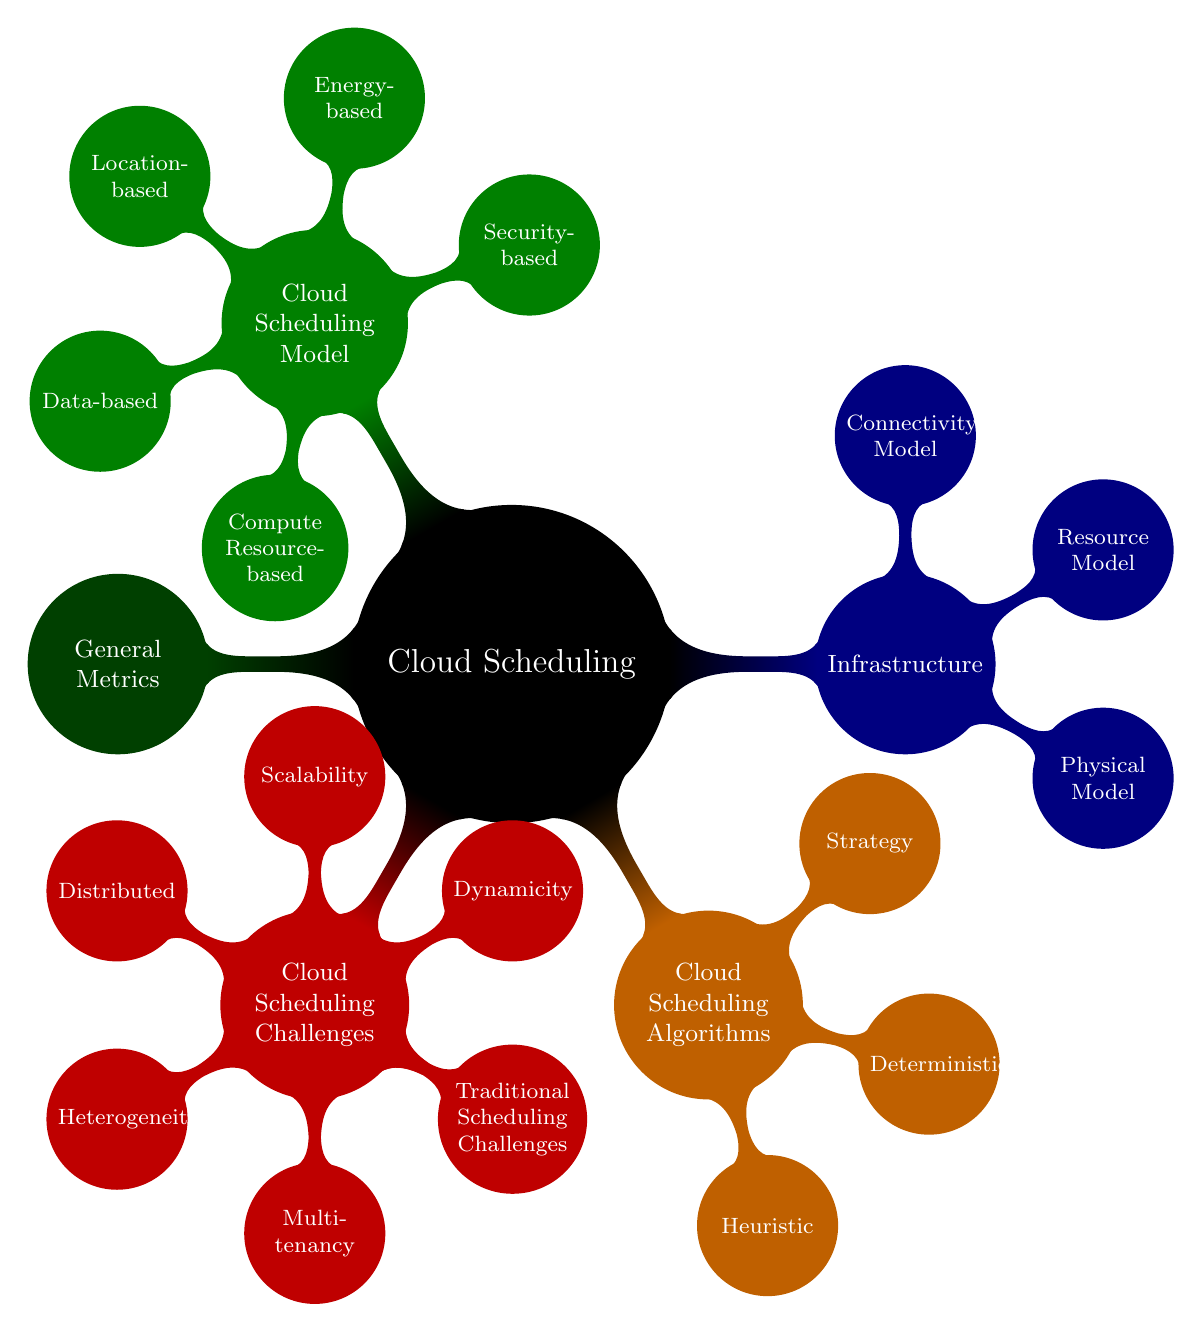
\begin{tikzpicture}
  \path[mindmap,concept color=black,text=white]
    
  node[concept] {Cloud Scheduling}
  [clockwise from=0]

  child[concept color=blue!50!black] {
      node[concept] {Infrastructure}
      [clockwise from=90]
      child { node[concept] {Connectivity Model} }
      child { node[concept] {Resource Model} }
      child { node[concept] {Physical Model} }
   }
  child[concept color=orange!75!black] {
      node[concept] {Cloud Scheduling Algorithms}
      [clockwise from=45]
      child { node[concept] {Strategy} }
      child { node[concept] {Deterministic} }
      child { node[concept] {Heuristic} }
   }
  child[concept color=red!75!black] {
      node[concept] {Cloud Scheduling Challenges}
      [clockwise from=-30]
      child { node[concept] {Diversity} }
      child { node[concept] {Multi-tenancy} }
      child { node[concept] {Heterogeneity} }
      child { node[concept] {Distributed} }
      child { node[concept] {Scalability} }
      child { node[concept] {Dynamicity} }
      child { node[concept] {Traditional Scheduling Challenges} }
  }
  child[concept color=green!25!black] {
      node[concept] {General Metrics}
  }
  child[concept color=green!50!black] {
      node[concept] {Cloud Scheduling Model}
      [clockwise from=-100]
      child { node[concept] {Compute Resource-based} }
      child { node[concept] {Data-based} }
      child { node[concept] {Location-based} }
      child { node[concept] {Energy-based} }
      child { node[concept] {Security-based} } 
   };
 \end{tikzpicture}
}
\end{figure}

\subsection{Resource Provider Focused Y-Cloud Taxonomy}\label{sec:y}

To showcase the interaction between the different layers more clearly we like to refer the reader to the Y-cloud scheduling diagram introduced by Laszewski in~\cite{lasbook}.

In this taxonomy, we are concerned about how resources are placed on physical models and are interconnected with each other to facilitate scheduling algorithms. Figure~\ref{F:graph-y} depicts the different models that are an integral part of this taxonomy. It includes the

\begin{description}

\item[Physical Model] representing major physical resource layers to enable a hierarchical scheduling strategy across multiple data centers, racks, servers, and computing cores.

\item[Resource Model] representing resource-based scheduling decisions while dealing with containers and functions, virtual machines and jobs, virtual clusters, provider-managed resources, and multi-region provider-managed resources.

\item[Connectivity Model] introducing connectivity between components when addressing scheduling. This includes components such as memory, processes, connectivity to distributed resources, hyper-graphs to formulate hierarchies of provider-based resources, and region enhanced hyper-graphs. The connectivity model allows us to leverage classical scheduling algorithms while applying such models and leveraging established or new scheduling algorithms for these models.

\end{description}

\begin{figure*}[p]
  \centering
  \resizebox{0.75\textwidth}{!}{%
  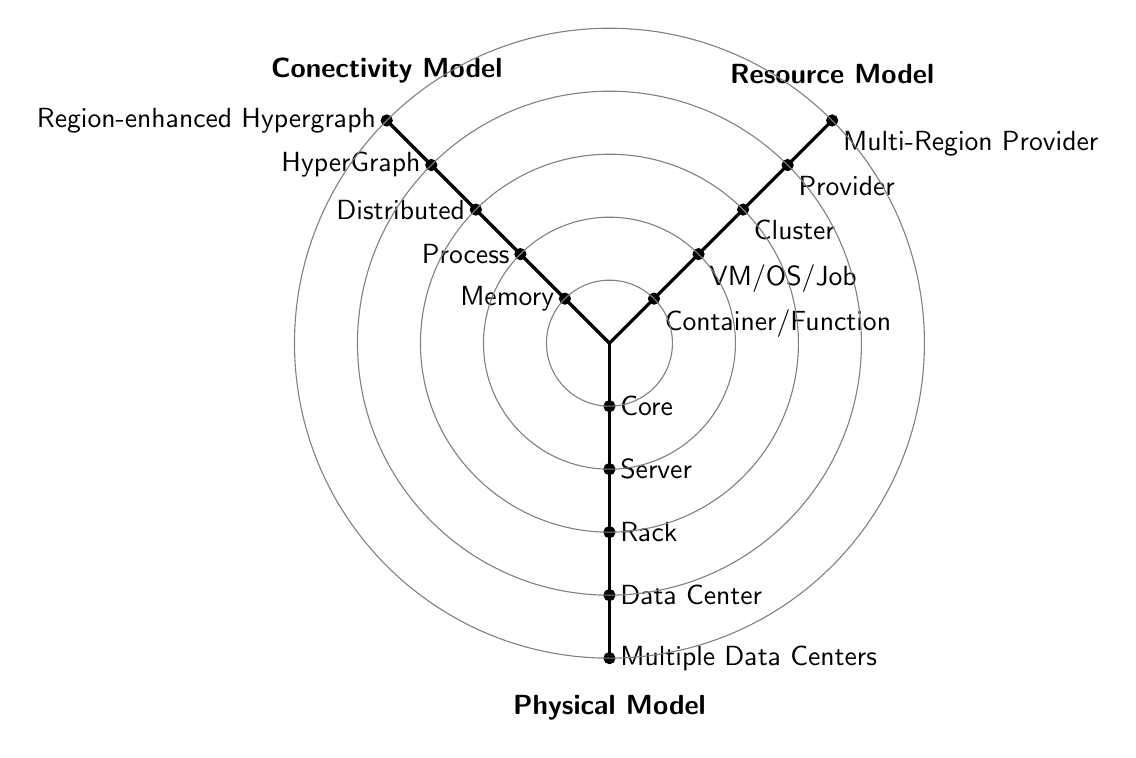
\begin{tikzpicture}[>=stealth',join=bevel,font=\sffamily,auto,on grid,decoration={markings,mark=at position .5 with \arrow{>}}]
  % \begin{tikzpicture}[>=stealth',join=bevel,font=\sffamily,auto,on grid,decoration={markings,mark=at position .5 with \arrow{>}}]
    %\input{y_chart_common}
    \coordinate (conectivityNode) at (135:4cm);
    \coordinate (resourceNode) at (45:4cm);
    \coordinate (physicalNode) at (270:4cm);
    \coordinate (originNode) at (0:0cm);

    \node [above=1em] at (conectivityNode) {\textbf{Conectivity Model}};
    \node [above=1em] at (resourceNode) {\textbf{Resource Model}};
    \node [below=1em] at (physicalNode) {\textbf{Physical Model}};

    \draw[-, very thick] (conectivityNode.south) -- (0,0) node[left,pos=0]{Region-enhanced Hypergraph} node[left,pos=0.2]{HyperGraph} node[left,pos=0.4]{Distributed} node[left,pos=0.6]{Process} node[left,pos=0.8]{Memory};

    \draw[-, very thick] (resourceNode.south) -- (0,0) node[pos=0]{Multi-Region Provider} node[pos=0.2]{Provider} node[pos=0.4]{Cluster} node[pos=0.6]{VM/OS/Job} node[pos=0.8]{Container/Function};

    \draw[-, very thick] (physicalNode.south) -- (0,0) node[right,pos=0]{Multiple Data Centers} node[right,pos=0.2]{Data Center} node[right,pos=0.4]{Rack} node[right,pos=0.6]{Server} node[right,pos=0.8]{Core};

    \draw[fill] (barycentric cs:conectivityNode=1.0,originNode=0) circle (2pt);
    \draw[fill] (barycentric cs:conectivityNode=0.8,originNode=0.2) circle (2pt);
    \draw[fill] (barycentric cs:conectivityNode=0.6,originNode=0.4) circle (2pt);
    \draw[fill] (barycentric cs:conectivityNode=0.4,originNode=0.6) circle (2pt);
    \draw[fill] (barycentric cs:conectivityNode=0.2,originNode=0.8) circle (2pt);

    \draw[fill] (barycentric cs:resourceNode=1.0,originNode=0) circle (2pt);
    \draw[fill] (barycentric cs:resourceNode=0.8,originNode=0.2) circle (2pt);
    \draw[fill] (barycentric cs:resourceNode=0.6,originNode=0.4) circle (2pt);
    \draw[fill] (barycentric cs:resourceNode=0.4,originNode=0.6) circle (2pt);
    \draw[fill] (barycentric cs:resourceNode=0.2,originNode=0.8) circle (2pt);

    \draw[fill] (barycentric cs:physicalNode=1.0,originNode=0) circle (2pt);
    \draw[fill] (barycentric cs:physicalNode=0.8,originNode=0.2) circle (2pt);
    \draw[fill] (barycentric cs:physicalNode=0.6,originNode=0.4) circle (2pt);
    \draw[fill] (barycentric cs:physicalNode=0.4,originNode=0.6) circle (2pt);
    \draw[fill] (barycentric cs:physicalNode=0.2,originNode=0.8) circle (2pt);

    \draw[black!50] (0,0) circle (4.0cm);
    \draw[black!50] (0,0) circle (3.2cm);
    \draw[black!50] (0,0) circle (2.4cm);
    \draw[black!50] (0,0) circle (1.6cm);
    \draw[black!50] (0,0) circle (0.8cm);
  \end{tikzpicture}
  }
  \caption{Resource Provider Focused Y-Cloud Taxonomy~\cite{las18cloudscheduling-whitepaper}.}
  \label{F:graph-y}
\end{figure*}


\subsection{Cloud Scheduling Model}

Now that we have identified the resource provider focused Y-Cloud taxonomy we can identify some important classifications that govern the scheduling decisions to effectively use these resources. This includes metrics that influence the scheduling. Traditional scheduling metrics and attributes for scheduling algorithms are shown in Figure~\ref{F:graph-metrics}. They include typically cost, time, space, reliability, energy, and security.


\begin{figure}[!th]
	\centering
\resizebox{0.6\columnwidth}{!}{%
\begin{forest}
skan tree
   [General Scheduling Metrics
        [Cost]
        [Time]
        [Space]
        [Reliability]
        [Energy]
        [Security]
   ]
]
\end{forest}
}
\caption{Traditional Compute Scheduling Metrics}
\label{F:graph-metrics}
\end{figure}


When looking into the specifics of these metrics applied to cloud computing we can easily identify more details for these traditional metrics that apply to the various infrastructure components that constitute a cloud including compute, data, energy, quality of service, and security. We depict some of the major attributes that influence the scheduling decisions in Figure~\ref{F:graph-taxonomy}. Furthermore, each of the attributes in the categories Compute, Data, Security, Energy, and Quality of service can be combined if not already included in the specific scheduling attribute. For example, to identify a scheduling model based on virtual machines, attributes such as those in data, energy, QoS, or security may be introduced in the scheduling decision.



\begin{figure}[!th]
	\centering
\resizebox{\columnwidth}{!}{%
\begin{forest}
skan tree
[Cloud\\ Scheduling Model
   [Compute-Resource-based
     [Workflow-based]
     [Job-based]
     [VM-based
       [Migration]
       [Placement]
     ]
     [Task-based]
     [Container-based]
     [Function-based]
     [Platform-based]
   ]
   [Data-based
        [Storage Type]
        [Volume]
        [Redundancy]
        [Network-based
          [Bandwidth]
          [Latency]
        ]
    ]
    [Location-based
            [Processor-based]
            [Server-based]
            [Room-based]
            [Datacenter-based]
            [Region-based]
            [Global-based]
        ]  
    [Energy-aware
        [HVAC]
        [Green IT]
        [PUE]
        [Energy Source]
    ]
    [Security-based
        [Public]
        [Private]
    ]
   ]
]
\end{forest}
}
\caption{Cloud Scheduling Models}
\label{F:graph-taxonomy}
\end{figure}





This information can now be used to define provisioning and service scheduling as categorized next.

\subsection{Challenges in Cloud Scheduling}\label{sec:challange}

It is important to understand that cloud scheduling is going beyond traditional scheduling approaches. For this reason, we need to look at specific challenges we face that will lead us to features that need to be addressed by scheduling solutions for the cloud and build significant requirements to be addressed by scheduling solutions

Some of the obvious cloud characteristics and challenges are listed next and are summarized in Figure~\ref{F:graph-challenges}.

\begin{description}

\item [Large scale:] Clouds offer a large number of resources to its users that need to be optimally utilized under the quality of service constraints set by providers and users. A cloud involving a plethora of resources spanning across the globe is obviously a huge infrastructure. The range of functions, tasks, jobs, and applications need to be scheduled at any point of time onto available resources. Handling them on such scale requires efficient resource management. As such, scheduling becomes a complex endeavor, integrating dynamic and multi-faceted scheduling. 

\item [Dynamic nature of clouds:] Clouds encompass a dynamically changing resource environment in which resources belong to different administrative domains keep on joining and leaving the clouds. Hence, scheduling must be adaptive and address the dynamic resource availability.

\item[Heterogeneous providers and services:] There is no single cloud. We have to recognize that the competitive nature in the cloud market promotes not only heterogeneous cloud providers but heterogeneous cloud services that may compete with each other and either offer the same or customized services targeting a particular user community. Resources in clouds are highly diversified in nature, capacity, working style, and administrative domains. The inclusion of different resource providers with the desire to lock customers into their services and products makes heterogeneous multi-cloud scheduling a formidable challenge.

\item [Highly diversified:] Due to the large diverse set of applications (but also infrastructure) smart strategies to schedule such applications on the required resources are needed.

\item [Decentralized:] The resources in the cloud are distributed among various data centers, rack, and servers. Although they may belong to a provider, they can still be utilized across provider boundaries and even within the same provider regions, calling for a high degree of decentralization.

\item[Limited control by users:] Due to the fundamental nature of the cloud, access to low-level scheduling mechanisms is often hidden and only available to the provider. On the other hand, users still have their own scheduling requirements in regards to, for example, cost and deadlines.
 
\item[Dynamic loads:] Due to the size of the user community sporadic burst on resource requirements lead to challenges to adjust provisioned resources and schedule application onto them.

\item[Security concerns:] Another important requirement for scheduling is the ability to integrate issues such as privacy and security considerations as the provider needs to assure that local laws, as well as, the general privacy and security concerns are addressed. This is especially of concern when government or health providers need to schedule resources in a cloud for their application needs, making it necessary to distinguish problems that can be executed on public vs private clouds through scheduling but also through policy decisions that integrate with scheduling algorithms.
 
\end{description}

Thus, we need to distinguish many scheduling challenges, one of which is governed by differentiating users and providers. Here, on the one hand, we focus on cloud providers that try to utilize in the best possible way to utilize the existing resources for the customers under optimization constraints such as cost, high availability, fault tolerance for the providing cloud resources and services. On the other hand, we have customers that expect quality assurances, but also have their own constraints such as deadlines, cost, and implicit requirements from their applications including data placement and management that may influence the scheduling decision.

In both cases, we need to address the challenge of provisioning resources and also the challenge of scheduling services onto these resources. Although they can be done independently, it is obvious that interrelationship between them is needed in case of re-provisioning and dynamic adaptation to dynamic loads placed on the resources.

In both cases under-utilization prevents a resource from performing optimally, incurring idle time, whereas over-utilization causes a resource to degrade the node's performance.


\begin{figure}[htpb]
  \centering
  \resizebox{1.0\columnwidth}{!}{%
\begin{forest}
skan tree
   [Cloud Scheduling Challenges
        [Diversity
           [Infrastructure]
           [Platforms]
           [Services]
        ]
        [Multi-tenancy]
        [Heterogeneity]
        [Distributed]
        [Scalability
           [Huge Infrastructure]
        ]
        [Dynamicity]
        [Traditional Challenges
          [Efficiency]
          [Cost]
          [Time]
          [Space]
          [Reliability]
          [Energy]
          [Security
            [Authentication]
            [Authorization]
            [Auditing]
            [Privacy]
          ]
        ]
   ]
]
\end{forest}
}
   \caption{Scheduling challenges applied to all levels} 
  \label{F:graph-challenges}
\end{figure}




%%%%%%%%%%%%%%%%%%%%%%%%%%%%%%%%%%%%%%%%%%%%%%%%%%%%%%%%%%
\subsection{Taxonomy Classification of Resource Scheduling Algorithms}\label{S:algo}
%%%%%%%%%%%%%%%%%%%%%%%%%%%%%%%%%%%%%%%%%%%%%%%%%%%%%%%%%%

Next, we present in Figure~\ref{F:graph-algorithm} a classification of resource scheduling algorithms that we found while reviewing a significant set of literature related to cloud computing. We focus in Figure~\ref{F:graph-algorithm} on a relevant subset while focussing on VM placement while considering QoS parameters to guide the scheduling task. An additional classification is based on the type of algorithm used for the scheduling task. Dependent on the locality and large scale of the scheduling task in many cases a deterministic approach is not suitable. Hence, different algorithm categories are listed in Figure~\ref{F:graph-scheduling}.

%When looking at heuristics~\cite{vivekanandan2011study}
%we find traditional algorithms such as hill-climbing but also a
%variety of nature-inspired algorithms. The detail description of
%existing work in the field of resource scheduling algorithm is done in
%the next section.


\begin{figure}[!thbp]
	\centering
\resizebox{1.0\columnwidth}{!}{%
\begin{forest}
skan tree
[Resource Scheduling Algorithms
      [Strategy
        [Parallelism
          [Batch]
          [Asynchronous]
        ]
        [Cooperation
          [Co-operative]
          [Non-cooperative]
        ]
      ]
      [Deterministic]
      [Heuristic
            [Nature Inspired
              [Simulated Annealing]
              [Genetic Algorithms]
              [Ant Colony Optimization]
              [Particle Swarm Optimization]
            ]
            [Tabu Search]
            [Hill Climbing]
      ]
]
\end{forest}
}
\caption{A subset of Resource Scheduling Algorithms}
\label{F:graph-algorithm}
\end{figure}

\begin{figure}[!th]
	\centering
\resizebox{1.0\columnwidth}{!}{%
\begin{forest}
skan tree
[Resource Scheduling Algorithms
    [VM Placement-based 
        [Dynamic VM placement]
        [Network aware VM placement]
        [Energy aware VM placement]
    ]    
    [Quality of Service-based 
            [Cost-based]
            [Time-based]
            [Reliability-based]
            [Security-based]
    ]
    [Heuristic-based]
    [Container-based]
    [Function-based ]
]
\end{forest}
}
\caption{Classification of Resource Scheduling Algorithms}
\label{F:graph-scheduling}
\end{figure}


%%%%%%%%%%%%%%%%%%%%%%%%%%%%%%%%%%%%%%%%%%%%%%%%%%%%%%%%%%
%%%%%%%%%%%%%%%%%%%%%%%%%%%%%%%%%%%%%%%%%%%%%%%%%%%%%%%%%%
%%%%%%%%%%%%%%%%%%%%%%%%%%%%%%%%%%%%%%%%%%%%%%%%%%%%%%%%%%
%%%%%%%%%%%%%%%%%%%%%%%%%%%%%%%%%%%%%%%%%%%%%%%%%%%%%%%%%%
%%%%%%%%%%%%%%%%%%%%%%%%%%%%%%%%%%%%%%%%%%%%%%%%%%%%%%%%%%
%%%%%%%%%%%%%%%%%%%%%%%%%%%%%%%%%%%%%%%%%%%%%%%%%%%%%%%%%%



%%%%%%%%%%%%%%%%%%%%%%%%%%%%%%%%%%%%%%%%%%%%%%%%%%%%%%%%%%
\section{Literature review of Cloud Resource Scheduling Algorithms}\label{sec:literature}
%%%%%%%%%%%%%%%%%%%%%%%%%%%%%%%%%%%%%%%%%%%%%%%%%%%%%%%%%%

In this section, we conduct an exemplary but extensive literature
review of cloud scheduling to confirm the {\bf taxonomy
 categories}. As part of this review, we present several tables to identify the categories from research and frameworks we reviewed and are related to cloud scheduling. We augmented each table with a first column that is highlighted and refers to the cloud scheduling taxonomy category we identified for this work.

To provide an additional guide we introduce several topical sections focusing and grouped the literature based on its main contribution to these groups. However, we avoided a double listing of the research in multiple groups as much as possible to keep the tables small.

As a result we organize this section by scheduling categories related to 
%
dynamic scheduling (Section~\ref{sec:dynamic}),
cloud metric-based scheduling with emphasize (Section~\ref{sec:vm-scheduling}) on 
energy (Section~\ref{sec:energy}),
network (Section~\ref{sec:network}),
cost (Section~\ref{sec:cost}),
time (Section~\ref{sec:time}),
reliability (Section~\ref{sec:reliability}),
security (Section~\ref{sec:security}), 
and heuristics (Section~\ref{sec:heuristic}).

As High-Performance Computing in the cloud is also a service offered by several providers, we also need to be aware of HPC in the cloud (Section~\ref{sec:hpc}) and scientific workflows (Section~\ref{sec:workflow}) that is going to become a field of interest for the scientific community. This is motivated by the fact that transition to cloud services takes place in academic and commercial settings and is explicitly an area of interest for NIST as discussed in the Big Data Reference Architecture Working Group while leveraging activities from the community including the past Grid community.

In this section, we also review papers with emphasis on scheduling in public clouds (Section~\ref{sec:public}), containers (Section~\ref{sec:container}), function as a service (Section~\ref{sec:faas}) as well as distributed resource providers (Section~\ref{sec:distributed}) which can utilize a service mesh (Section~\ref{sec:mesh}).





\subsection{Dynamic Scheduling}\label{sec:dynamic}

In literature, we find the distinction between static and dynamic cloud scheduling algorithms. In static scheduling, resources are scheduled once, while in dynamic scheduling updates are applied constantly to find better resource utilization during runtime.


The latter is often motivated by the need for scalability~\cite{keller2014hierarchical} across and within data centers or increased fault tolerance~\cite{tighe2013distributed}. Association of other metrics into the dynamic scheduling approach is common while including power, network bandwidth and the integration of sophisticated service level agreements~\cite{tighe2013distributed}.

In many cases, not only the cloud user but also the cloud provider can benefit from dynamic scheduling~\cite{tighe2014integrating}.

We find that it can be beneficial to separate the scheduling task in multiple steps such as shown in~\cite{sun2015live}. Here, live migration for correlated VMs is optimizing on data, compute, and bandwidth conducted in several steps. Other cloud metrics such as price~\cite{tordsson2012cloud} are also common and will be addressed in Section ~\ref{sec:cost}. To address the scale problem many such algorithms use heuristics as showcased in Section~\ref{sec:heuristic}.

Table~\ref{T:dynamic-scheduling} lists several efforts related to dynamic scheduling while focusing on virtual machine placement.


%\newcolumntype{g}{>{\columncolor{Gray}}p}
\begin{table*}[!htbp]
 \caption{Comparison of Dynamic Scheduling Algorithms}
     \label{T:dynamic-scheduling}
   \centering
\scriptsize
\resizebox{\textwidth}{!}{%
\begin{tabular}{|g{2cm} p{2cm} p{2cm} p{2cm} p{2cm} p{2cm} p{2cm} p{1.5cm}|}
  \hline
 \textbf{Taxonomy Classification} & \textbf{Author} & \textbf{Basis} & \textbf{Advantages} & \textbf{Disadvantages} & \textbf{scheduling techniques} & \textbf{Experimental Scale} &\textbf{Experimental Parameters}

\\ \hline

 Energy-basedd, energy source & Sun et al.~\cite{sun2015live} & Introduction of a virtual data center to solve VM migration issues & Low complexity & Fixed band-with & Heuristic algorithm & Simulated environment & VM migration cost and time
\\ \hline

Energy-basedd, VM migration & Tighe et al.~\cite{tighe2014integrating} & Auto scaling  algorithm  alongside  a  dynamic VM  allocation  algorithm  & Reduce a number of migrations & No optimization criteria &Rule based heuristic&  DCSim & Power, SLA, Migrations 
\\ \hline

Energy-based & Keller et al.~\cite{keller2014hierarchical} &  Management of data center resources to reduce the management scope &  Reducing  the  overhead  in  the  data centre management network & High complexity & Greedy algorithm & DCSim  & Power, number of migrations, average number of racks, active hosts 
\\ \hline 

Energy-based, PUE & Tighe et al.~\cite{tighe2013distributed} &  Trade-off  among number of  migrations, SLA  violation and power & Consider energy and SLA & more bandwidth usage & First fit algorithm &  DCSim  & Power consumption, number of migrations, SLA violations 
\\ \hline 

Compute-resource based, VM based & Tordsson et al.~\cite{tordsson2012cloud} &  Optimized placement of applications in multi-cloud environments & Emphasized on Price and performance in terms of hardware configuration, load balancing & Ignored security and energy efficiency at time of scheduling & Integer programming formulations & Amazon EC2 & Throughput, number of jobs 
\\ \hline


Energy-based, VM-based & Younge et al.~\cite{las10cloudsched} & 
Power aware & 
reduces cost & 
slight reduction in performance & 
heuristic & on premise cloud & 
power consumption 

\\ \hline

\end{tabular}
}
\end{table*}




\subsection{Cloud Metric-based Scheduling}\label{sec:vm-scheduling}

Due to the complexity of cloud environments, many different metrics are used to guide the scheduling of virtual machines, containers, platforms, tasks, batch jobs, and workflows (see Figure~\ref{F:graph-metrics}). Next, we review examples of literature that integrates such metrics into their scheduling algorithm.


% Figure ~\ref{F:graph-metrics-flower} showcases
% 
\begin{figure}[phtb]
  \centering
  \resizebox{0.5\columnwidth}{!}{%
\smartdiagram[bubble diagram]{Scheduling Metrics, Cost, Time, Security, Energy, Reliability}
}
   \caption{Multi-phase scheduling in a hierarchical resource model} 
  \label{F:metrics}
\end{figure}


\subsubsection{Energy Aware Scheduling}\label{sec:energy}

Energy consumption is a key issue for cloud providers due to the enormous cost associated with operating hyper-scale and large cloud data centers. By using server consolidation, optimizing operation on physical machines, energy consumption can be reduced in contrast to smaller-scale infrastructure. Also, while using dynamic voltage scaling of processors, energy consumption can be reduced as shown in~\cite{las09dvfs,las10dvfs,calheiros2014energy} by slowing down the services.

Various scheduling methods such as to minimize the total makespan~\cite{bessis2013using}, developing dynamic meta-heuristics~\cite{bi2017application}, fractal mathematics~\cite{duan2016energy}, and machine learning clustering and stochastic~\cite{bui2017energy} have been utilized to optimize energy-aware scheduling. Multiple metrics must be included to correlate, for example CPU, RAM, and bandwidth~\cite{zhu2017three}.

These features, for example, could be utilized to dynamically adapt to peak loads~\cite{duan2016energy} while making processors faster during such periods. Furthermore, migration~\cite{beloglazov2010energy} has naturally an impact on energy cost. Energy cost in multi-cloud and hybrid-cloud data centers in the clouds are discussed in~\cite{quarati2013hybrid,garg2011environment,gai2016dynamic,dabbagh2015energy} while at the same time increasing the cloud provider broker’s revenue.


Others create models to predict the energy consumption of each virtual machine~\cite{kim2014energy}. This requires the ability to properly monitor the underlying server farms in a cloud data center as discussed in~\cite{van2012comparison}. Integration of historical or previous program executions while recording their energy consumption can also be utilized~\cite{hu2010scheduling}. Others focus on predicting future resource consumption needs~\cite{dabbagh2015energy}.

A comparison of energy-aware scheduling algorithms in cloud computing is shown in Table~\ref{T:g-a} and \ref{T:g-b}.



%\begin{sidewaystable*}[!htbp]

\caption{Comparison of Energy-aware VM Placement-based Scheduling
  Algorithms (A)}\label{T:g-a}
 \hspace{8pt}
\centering
\scriptsize
\resizebox{\textwidth}{!}{%
\begin{tabular}{|g{2.1cm} p{1.5cm} p{2cm} p{2cm} p{2cm} p{2cm} p{2cm} p{2cm}|}
  \hline
  % after \\: \hline or \cline{col1-col2} \cline{col3-col4} ...
\textbf{Classification} & \textbf{Author} & \textbf{Basis} & \textbf{Advantages} & \textbf{Disadvantages} & \textbf{scheduling techniques} & \textbf{Experimental Scale} &\textbf{Experimental Parameters} 
\\ \hline

  \makecell{Energy source, \\Compute\\ resource-based, \\Job-based} & Calheiros et al.~\cite{calheiros2014energy} & Intelligent scheduling combined DVFS capability  &  Improved energy efficiency  & Ignored Network and Storage energy consumption  &  Rank method   & Cloud Sim & Energy consumption
\\ \hline 

\makecell{Energy-aware, \\PUE} & Bessis et al.~\cite{bessis2013using} & Improving communication for Distributed systems at the time of scheduling & Improved system performance & High complexity & Graph theory concepts & SIMIC & makespan, latency times 
\\ \hline 
  
\makecell{Energy-aware,\\ Energy source, \\Cost, \\VM-based} & Bi et al.~\cite{bi2017application} & Dynamic Scheduling algorithm for reducing energy consumption & Focused on performance and energy cost & High complexity due to virtualized Data centers & meta heuristic methods & Simulated environment & Profit, CPU utilization  
\\ \hline   

    \makecell{Energy-aware,\\ Compute\\ resource-based, \\VM-based} & Duan et al.~\cite{duan2016energy} & Scheduling of VM machines & Improved the CPU load prediction & No optimization & Ant colony optimization &  CloudSim & Energy Consumption
\\  \hline 

  \makecell{Energy-aware,\\ Energy source,\\ Cost, \\VM-based} & Bui  et al.~\cite{bui2017energy} & Balance between energy efficiency and quality of service & Low complexity & Ignored cost, scalability & Greedy first fit algorithm & Simulated Environment & Energy, Memory, CPU  
\\ \hline


\makecell{Energy-aware,\\ Energy source, \\ Cost,\\ VM-based} & Zhu et al.~\cite{zhu2017three} & Data center balance while saving power consumption & Improved management of VM resource & High complexity &  Multi-dimensional vector bin packing problem-based heuristic & CloudSim & SLA violations, Resource utilization
\\ \hline

\makecell{Energy-aware, \\ Energy source,\\ VM-based} & Beloglazov et al.~\cite{beloglazov2010energy} &  Enhancement of resource utilization by re-allocation of the resources. & Considered different types of workloads, No prior information about applications & Ignored cost and time & Heuristic algorithm & CloudSim & Energy, Average SLA, migrations
  \\ \hline

  
\makecell{Energy source,\\ Compute\\ resource-based , \\VM-based}  & Quarati et al.~\cite{quarati2013hybrid} &  Reservation of a quota of private resources & Reduced energy consumption and carbon emission & Lacks implementation on a real-world cloud platform & Round robin algorithm & Discrete Event Simulator & User satisfaction, energy saving, energy consumption
\\ \hline

  \makecell{PUE, \\ Job-based} & Garg et al.~\cite{garg2011environment} &  Optimal scheduling policies & Reduced energy cost, energy consumption & Ignored security & Meta-scheduling policies & Simulated environment  & Average energy consumption, average carbon emission, arrival rate of application
 \\ \hline
 

\end{tabular}
}
\end{sidewaystable*}
  

 \begin{sidewaystable*}[!htbp]

   \caption{Comparison of Energy-aware VM Placement-based Scheduling Algorithms (B)}\label{T:g-b}
   \hspace{8pt}
  
\centering
\scriptsize
\resizebox{\textwidth}{!}{%
\begin{tabular}{|g{2cm} p{1.5cm} p{2cm} p{2cm} p{2cm} p{2cm} p{2cm} p{2cm}|}
  \hline
  % after \\: \hline or \cline{col1-col2} \cline{col3-col4} ...
\textbf{Classification} & \textbf{Author} & \textbf{Basis} & \textbf{Advantages} & \textbf{Disadvantages} & \textbf{scheduling techniques} & \textbf{Experimental Scale} &\textbf{Experimental Parameters} 
   
\\ \hline

\makecell{Energy-aware,\\ VM-based} & Keke et al.~\cite{gai2016dynamic} & Cloudlets for energy reduction & Reduced energy consumption & No time consideration & FCFS scheduling policy & DECM-Sim & Energy consumption 
\\ \hline
  
\makecell{Energy source,\\ VM-based} & Dabbagh et al.~\cite{dabbagh2015energy} &  Energy-aware resource management decisions  & improved performance & No optimization criteria, high complexity& K-means clustering& Testbed & Average CPU and Network utilization
\\ \hline

    \makecell{Energy source, \\VM-based} & Kim et al.~\cite{kim2014energy} & VM energy consumption estimation model & Reduced cost, power consumption & More complex to implement, Ignored time & Power aware scheduling algorithm & Xen 4.0 hypervisor & Energy consumption, error rate
\\ \hline

\makecell{Compute\\ resource-based,\\ VM-based} & Van Do et al. in~\cite{van2012comparison} & Interaction aspects between on-demand requests and the allocation of virtual machines & Reduced energy consumption & No cost and time optimization & Power aware scheduling algorithm & Numerical Simulation & Average Energy consumption, average heat emission
\\ \hline

  
  \makecell{Energy-aware,\\ Energy source, \\Compute \\resource-based, \\
  VM-based (migration),\\ Workflow} & Li et al.~\cite{li2016energy} & Scheduling algorithm to reduce energy consumption while meeting the deadline constraint & Focused on energy consumption & Ignored  processing power energy consumption, VM migration & Heuristic method & Simulated environment & Energy consumption
\\ \hline 


  \makecell{Energy source,\\PUE, \\ VM-based} & Ding  et al.~\cite{ding2015energy} & Dynamic VMs scheduling & Increased Processing Capacity & Ignored VM migration, Power penalties of status transitions of processor & FCFS & Simulated environment  & Deadline, Energy consumption 
\\ \hline 



\end{tabular}
}
\end{sidewaystable*}


\subsubsection{Network Aware Scheduling}\label{sec:network}

Clouds promote large-scale network traffic to, from, and within clouds. Thus network-aware scheduling must be considered for scheduling. This not only contains moving data in and out of the cloud data center but may also contain message exchanges between complex distributed applications that run in cloud data centers in a distributed fashion.

Minimizing the distance between data providers and data consumers while, for example,replicating data~\cite{www-akamai} can save a significant amount of traffic and has long been applied on the internet as one of its beneficial strategies. Service level agreements (SLA)~\cite{breitgand2012improving} are playing an important role to achieve proper utilization as part of the scheduling effort. Treating the network as shared scarce resource~\cite{rampersaud2016sharing} motivates the development of network-based scheduling algorithms. Also in network-aware scheduling, we find the distinction between static~\cite{biran2012stable} and dynamic scheduling at runtime so we can deal with traffic bursts.

A variety of traditional scheduling metrics (see Figure~\ref{F:graph-metrics}) are often used to improve scheduling while considering network traffic. An example is demonstrated in ~\cite{yu2017survivable} to optimize traffic in virtual clusters. Scheduling across multiple layers is especially of benefit for networking~\cite{bi2015sla}. Scheduling of platforms such as Hadoop, offers advantages when networking is integrated~\cite{kondikoppa2012network}. Having access to lower-level infrastructure such as offered by OpenStack, presents opportunities to include Network Function Virtualization (NVF)~\cite{lucrezia2015introducing}.

Table \ref{T:c} shows examples of network-aware scheduling algorithms in cloud computing.



%  \begin{sidewaystable*}[p]
\caption{Comparison of Network-aware VM Placement-based Scheduling Algorithms}\label{T:c}
\centering
\scriptsize
\resizebox{\textwidth}{!}{%
\begin{tabular}{|g{2cm} p{2cm} p{2cm} p{2cm} p{2cm} p{2cm} p{2cm} p{1.9cm}|}
  \hline
   \textbf{Classification} & \textbf{Author} & \textbf{Basis} & \textbf{Advantages} & \textbf{Disadvantages} & \textbf{scheduling techniques} & \textbf{Experimental Scale} &\textbf{Experimental Parameters} 
   
\\ \hline

VM based & Yu et al.~\cite{yu2017survivable} & Service provisioning on IaaS platform while focusing on the inter-connected
VMs. &  High availability & High complexity & Heuristic algorithm & Simulator & Average VM consumption ratio, average running time 
\\ \hline 

Compute resource based, VM based & Bi et al.~\cite{bi2015sla}~\cite{bi2016trs} & Architecture for self management of data centers & Considered temporal request of multi-tier web applications  & does not consider security parameters  & Queuing approach &  trace-driven simulation & Cost 
\\ \hline

 Compute resource based & Rampersaud et al.~\cite{rampersaud2016sharing} & Used page-sharing concept to handle VM Packing problem & Improvement of memory sharing during allocation decisions & High complexity & Linear programming technique & Simulated environment & Memory reduction, number of excess servers 
\\ \hline

 Compute resource-VM based & Lucrezia et al.~\cite{lucrezia2015introducing} & Investigated OpenStack for the deployment of network service graphs & Increased throughput & Analyzing time is more, Ignored policy-constraints in  order  to  define  administration  rules&  Brute force algorithm  & KVM hypervisors &  VM locations, traffic throughput and latency 
\\ \hline 

Compute resource VM based & Biran et al.~\cite{biran2012stable}& Consideration of traffic  bursts  in  deployed  services & Minimizing  the  maximum load  ratio  over  all  the  network & Ignored energy consumption& Greedy heuristic algorithm & Testbed & Average packet delivery delay , placement solving time  
\\ \hline




Compute-resource based workflow based & Kondikoppa et al.~\cite {kondikoppa2012network} & To make Hadoop scheduler aware of network topology & Improved data locality& Ignored cost, energy, security & FIFO &Eucalyptus  based testbed & Execution time, delay for scheduling task 


\\ \hline

\end{tabular}
}
\end{sidewaystable*}



\subsubsection{Cost Aware Scheduling}\label{sec:cost}

Cost in clouds arises by using the data center facilities. These costs are passed along to the users.

Through shared use of the facilities and keeping under-utilization low, clouds can have an advantageous cost-performance ratio compared to on-premise compute and data centers. Costs for such centers include hardware operation, costs such as energy and equipment, as well as, operating costs, such as software licensing and update and personnel costs. Dependent on the hardware and software used, cloud providers offer a tiered cost model that allows users to assess the need for data, speed, and reliability as part of their cost analysis. Other options such as the selection of renewable energy use within the data center in case of energy conscious customers may also play a role.

Cost aware scheduling has been applied to virtual machines~\cite{yuan2017ttsa}, tasks~\cite{yuan2017temporal,zuo2015multi}, workflows~\cite{arabnejad2015cost,arabnejad2016budget}, as well as high-throughput~\cite{yuan2016cawsac} computing and use of data placement. Revenue maximization~\cite{yuan2018warm} has not only been applied to metrics such as latency~\cite{ghahramani2017toward}, but is also useful via advanced Dynamic Voltage and Frequency Scaling (DVFS)~\cite{las10cloudsched,calheiros2014energy} due to reducing the high energy costs with little performance reduction. This also could be achieved through delayed execution~\cite{bi2016trs} or relaxation of deadlines~\cite{zhang2018dynamic}. Other strategies include the introduction of penalties as part of SLA~\cite{wu2012sla}. Typical resource utilization such as optimizing processor sharing~\cite{lee2012profit} data placements~\cite{lee2012profit}, have been known to decrease cost. Also, dynamic adaptations at run-time allow reduction of cost~\cite{ari2013design}

To allow customers to decide the usage of various services including compute, data, function, and platform, most publish extensive cost schemes that can then be integrated into customers scheduling decisions.

Table \ref{T:e} presents a comparison of cost-aware scheduling algorithms.

%%\begin{sidewaystable*}[p]
\begin{table}[htb]
\caption{Comparison of Cost-based Scheduling Algorithms}\label{T:e}
\hspace{8pt}
\centering
\scriptsize
\resizebox{\textwidth}{!}{%
\begin{tabular}{|g{2cm} p{2cm} p{2cm} p{2cm} p{2cm} p{2cm} p{2cm} p{1.9cm}|}
  \hline
   \textbf{Classification} & \textbf{Author} & \textbf{Basis} & \textbf{Advantages} & \textbf{Disadvantages} & \textbf{scheduling techniques} & \textbf{Experimental Scale} &\textbf{Experimental Parameters} 

\\ \hline                                                                                                                                                                              
                                                                                                                                                                              
  \makecell{Compute\\ resource-based,\\ Task-based,\\ Cost-based} & Bi et al.~\cite{bi2015sla}~\cite{bi2016trs} & Architecture for self management of data centers & Considered temporal request of multi-tier web applications  & does not consider security parameters  & Queuing approach &  trace-driven simulation & Cost
  \\ \hline
  
\makecell{Compute\\ resource-based,\\  data-based,\\  task,\\  Latency,\\  VM-based,\\ Cost-based} & Yuan et al.~\cite{yuan2017ttsa,yuan2017temporal} & Emphasizing profit maximization & handles service delay bound & High complexity  & PSO and SA & simulation environment & Revenue
\\ \hline

\makecell{Compute\\ resource-based,\\  Task-based,\\ Cost-based}  & Zuo et al.~\cite{zuo2015multi} & Multi-objective Task Scheduling  & Improved  performance & Ignored energy consumption & Ant colony optimization & CloudSim & Cost, makespan, deadline violation rate
\\ \hline

\makecell{Compute\\ resource-based,\\  Workflow-based,\\ Cost-based} & Arabnejad et al.~\cite{arabnejad2015cost} &  Re-use of pre-provisioned instances for scheduling & Less complexity& Ignored security and energy efficiency& Deadline early Tree algorithm & CloudSim & Cost and deadline
\\ \hline

\makecell{Compute\\ resource-based,\\ VM-based,\\ Cost-based} & Wu et al.~\cite{wu2012sla} &  VM usage efficiency designed utility function by considering dynamic VM deploying time, processing time and data transfer time & Improved cost saving & Does not support security and energy efficient  & Admission control and scheduling algorithm & CloudSim & Average response time, total profit
\\ \hline

\makecell{Data-based,\\ Cost-based} & Lee et al.~\cite{lee2012profit} &  Personalized
features of the user request and the elasticity of SLA properties & Reduced operational costs and increase profits & Objectives conflict with each other & binary integer programming & CloudSim & Average utilization, average net profit rate, average response time  
  \\ \hline


\makecell{Compute\\ resource-based,\\  VM-based,\\ Cost-based} & Ari et al.~\cite{ari2013design} &  Finite Element Analysis cloud service with a focus on mechanical structural analysis, performance characterization and job scheduling issues & Throughput improvement and resource utilization & Ignored cost& Adaptive algorithm & Testbed & Throughput and time
\\ \hline

  
\end{tabular}
}
\end{table}
%\end{sidewaystable*}


\subsubsection{Time-based Scheduling}\label{sec:time}


Cloud users have the desire to reduce the time it takes to execute their applications and fulfill deadlines~\cite{arabnejad2017scheduling}. Besides virtual machine and time-based scheduling, it is also important to integrate data-aware scheduling to reduce access time to the data~\cite{vandenbosshe2013}. Historical data~\cite{thomas2015credit} or proxies~\cite{erdil2013autonomic} for execution times help designing time-aware scheduling algorithms. We find algorithms that integrate deadline constraints ~\cite{li2016energy}, completion time~\cite{xu2011job} with fairness, low downtime to improve time for execution~\cite{frincu2014scheduling}, and delay bounds ~\cite{yuan2017time}.

Table~\ref{T:f} presents a comparison of time-aware scheduling algorithms.

%\begin{sidewaystable*}[!htbp]
   \caption{Comparison of Time-based Scheduling Algorithms}
    \label{T:f}
\centering
\scriptsize
\resizebox{\textwidth}{!}{%
\begin{tabular}{|g{2cm} p{1.9cm} p{2cm} p{2cm} p{2cm} p{2cm} p{2cm} p{2cm}|}
  \hline
  % after \\: \hline or \cline{col1-col2} \cline{col3-col4} ...
 \textbf{Classification} & \textbf{Author} & \textbf{Basis} & \textbf{Advantages} & \textbf{Disadvantages} & \textbf{scheduling techniques} & \textbf{Experimental Scale} & \textbf{Experimental Parameters} 
 
\\ \hline

Compute-resource based, task & Yuan et al.~\cite{yuan2017time} & Task scheduling in green data centers & Investigated temporal variations &  Ignored energy consumption and cost & PSO and SA & Simulated Environment & Delay bound and time 
\\ \hline

 Compute resource based workflow & Arabnejad et al.~\cite{arabnejad2017scheduling} & Dynamically provisioned commercial cloud environments & Evaluation of task selection algorithms reveals impact of workflow symmetry & High complexity & Rank method & CloudSim & Response time, Cost 
\\ \hline

Compute-resource based, Workflow & Thomas et al.~\cite{thomas2015credit} & Task length aware scheduling & Lesser makespan and increased resource utilization & No comparison with existing algorithm & Min-min & CloudSim & Makespan 
\\ \hline 

Compute-resource based, VM & Frincu~\cite{frincu2014scheduling} & A priory scheduling and  searching for an optimal allocation of components on nodes in order to ensure a homogeneous spread of component types on every node. & Minimizing the application cost & Centralized approach represents a single point of failure & Nonlinear-programming & Simulator platform & Average load per node, optimal allocation, reliability 
\\ \hline

Compute-resource based, VM & Erdil~\cite{erdil2013autonomic} & Disseminated information as agents of dissemination sources for resource scheduling & Availability of resource state, reduces dissemination overhead & Ignored cost as parameters & Adaptive proxy algorithm & Scalable simulation network framework & Query satisfaction rates, random walk hop count limit 
\\ \hline


 Compute-resource based, Data based, Task-based & Van den Bossche et al. in~\cite{vandenbosshe2013} & Deadline-based workloads in a hybrid cloud setting & Minimize cost and time & does not handle multiple workflows & hybrid scheduling approach & Simulator & Total Cost, application deadline met, turnaround time, data transferred 
\\ \hline

Compute-resource based , task & Xu et al.~\cite{xu2011job} & Berger model and assign tasks on optimal resources to meet user's QoS requirements & Optimal completion time & Ignored cost and energy efficiency, security& Resource allocation algorithm and then followed by job scheduling & CloudSim & Time, bandwidth 
\\ \hline


\end{tabular}
}
\end{sidewaystable*}


\subsubsection{Reliability Aware Scheduling}\label{sec:reliability}



Cloud Users and providers need the guarantee of reliability. Thus, many cloud scheduling efforts address how to increase reliability. Strategies such as replication of data and compute services are common practice. This often comes at a price and increased cost may occur when reliability is of concern. The distributed nature of clouds makes it a formidable challenge to offer reliability. However at the same time, while providing (a) large scale data centers to offer cloud services with (b) highly specialized operating staff and (c) abilities to replicate and migrate workloads to other services, it increases reliability when compared to on-premise data centers. This is often due to the larger efficiency of the cloud data centers regarding the overall cost for its users.

Various studies have been conducted to analyze the effect of reliability on clouds.

This includes reliability assessment models ~\cite{malik2012reliability}, integration of communication and networks~\cite{jing2015reliability}, increase of resource availability~\cite{latiff2016fault}. Trade-offs between different scheduling metrics such as energy and reliability have also been studied~\cite{tang2016energy}.

A comparison of reliability and scheduling is given in Table~\ref{T:h}.

%\begin{sidewaystable*}[!htbp]
\caption{Comparison of Reliability-based Scheduling Algorithms}\label{T:h}
\hspace{8pt}
\centering
\scriptsize
\resizebox{\textwidth}{!}{%
\begin{tabular}{|g{2cm} p{2cm} p{2cm} p{2cm} p{2cm} p{2cm} p{2cm} p{1.9cm}|}
  \hline
   \textbf{Classification} & \textbf{Author} & \textbf{Basis} & \textbf{Advantages} & \textbf{Disadvantages} & \textbf{scheduling techniques} & \textbf{Experimental Scale} &\textbf{Experimental Parameters} 
\\ \hline

\makecell{Compute\\ resource-based,\\ Job-based,\\ Reliability-based} & Malik et al.~\cite{malik2012reliability} & Reliability assessment mechanism for scheduling resources & Reliability assessment algorithms for general applications and real time applications  & No security and energy parameters consideration & Max -min & Amazon EC2 cloud & Fault tolerance, time
\\ \hline

\makecell{Compute\\ resource-based,\\ Job-based,\\ Reliability-based} & Jing et al.~\cite{jing2015reliability} &  Model for fault-tolerant aware scheduling &  Low complexity  & No cost, time optimization & Adaptive secure scheduling algorithm & Simulated environment & Reliability
\\ \hline
  
\makecell{Compute\\ resource-based,\\ Task-based,\\ Reliability-based} & Abdulhamid et al.~\cite{latiff2016fault} & Uncountable numeric nodes for resource in clouds & Lower makespan & No optimization & League championship algorithm & CloudSim & Failure ratio, the failure slowdown and the performance improvement rate
\\ \hline

\makecell{Energy-aware ,\\ Energy source,\\ Reliability-based} & Tang et al.~\cite{tang2016energy} &  Reliability and energy-aware task scheduling architecture & To get good trade off among performance, reliability, and energy consumption & No support for cost optimization& Heuristic method & Discrete event simulation environment  & Schedule length, Energy consumption,  Application reliability 
 \\ \hline


\end{tabular}
}
\end{sidewaystable*}


\subsubsection{Security-based Scheduling}\label{sec:security}


Security is a key feature cloud users and providers require for cloud infrastructure to be useful for many applications.

Virtual machine scheduling requires the need for isolation, that can be controlled by security policies~\cite{afoulki2011security}. Isolation can also apply to the incoming and outgoing data~\cite{chejerla2017qos,kashyap2014security}. Risks occurring by inspecting the connections among VMs ~\cite{shetty2016security} can be analyzed and integrated into scheduling strategies. To enable trust between components in the cloud key exchanges have been proposed~\cite{liu2013ccbke}.

Multiple possibly contradictory scheduling objectives need to be also considered in many scheduling frameworks.

An example included the cost it takes to provide security and integrate it adequately in security scheduling frameworks~\cite{kashyap2014security,zeng2015saba,wang2012cloud}. Furthermore, as many edge devices need to interface with cloud services due to their computational and data limitations, privacy-preserving solutions to interface between clouds and mobile and edge devices have been considered ~\cite{bilogrevic2011meetings}.

Security-based scheduling algorithms are presented (see Table~\ref{T:i}).



%\newcolumntype{g}{>{\columncolor{Gray}}p}
\begin{table*}[!htbp]
\caption{Comparison of Security based Scheduling Algorithms}
     \label{T:i}
\centering
\scriptsize
\resizebox{\textwidth}{!}{%
\begin{tabular}{|g{2cm} p{2cm} p{2cm} p{2cm} p{2cm} p{2cm} p{2cm} p{1.9cm}|}
  \hline
  \textbf{Taxonomy Classification} & \textbf{Author} & \textbf{Basis} & \textbf{Advantages} & \textbf{Disadvantages} & \textbf{scheduling techniques} & \textbf{Experimental Scale} & \textbf{Experimental Parameters} 

\\ \hline

Compute-resource and Data based  & Chejerla et al.~\cite{chejerla2017qos} &  Scheduling of resources in cloud integrated Cyber-physical Systems & Consideration of security, time & High complexity &Heuristic algorithm & Simulated environment & Speed up, resource utilization, makespan 
\\ \hline

Compute-resource based, VM based & Shetty et al.~\cite{shetty2016security}& VM placement techniques to reduce security risks & Reduced computing costs and deployment costs& No optimization criteria & Heuristic algorithm& Simulated environment & Cost, security risks & 
\\ \hline 

Compute resource based-workflow & Zeng et al.~\cite{zeng2015saba} & Scheduling algorithm for resource utilization & Low complexity & Ignored energy consumption & Clustering and prioritization algorithm  &  Simulated environment & Makespan and speed up 
\\ \hline 

Compute-resource based, VM based & Kashyap et al.~\cite{kashyap2014security}& Secure aware scheduling of real time based applications & Improved response time and overall security & High complexity & Priority Algorithm & Hypervisor & Deadline, Security 
\\ \hline 

Compute-resource based, Workflow & Liu et al.~\cite{liu2013ccbke} &  Scheme for security aware scheduling &  Reduced the computational load and execution time  & No cost optimization involved & Adaptive secure scheduling algorithm & KVM hyper-visor & Time unit consumed per computational load 
\\ \hline

Compute-resource based, Task based & Wang et al.~\cite{wang2012cloud} & Uncountable numeric nodes for resource in clouds& Provided scheduling of resources in secure way & Ignored cost & Bayesian  algorithm& CloudSim & Trust value, average schedule length 
\\ \hline

Compute-resource based, VM based & Afoulki et al.~\cite{afoulki2011security}& Security risk management in a cloud &  Less complexity & Consolidation issues while implementing policies & Greedy Algorithm & Simulated environment & VM placement time  
\\ \hline 

Compute-resource based, VM based & Bilogrevic et al.~\cite{bilogrevic2011meetings} & Scheduling services on the cloud for mobile devices & Enhanced Performance & No support cost optimization, Ignores power consumption by the network & Privacy aware scheduling schema & Testbed & Time, Data exchanged, privacy in approach 
 \\ \hline
\end{tabular}
}
%\tiny}

\end{table*}


\subsection{Heuristic-based Scheduling}\label{sec:heuristic}


Heuristic methods help to design efficient algorithms in the case where deterministic methods can not be applied. We provide here a small sample of heuristics applied to clouds as found in the literature. This includes particle swarm optimization~\cite{pandey2010particle}, multi-objective genetic algorithm-based ~\cite{mezmaz2011parallel,gkasior2016metaheuristic}, colony optimization with swarm intelligence~\cite{mateos2013aco}, bee colony~\cite{ld2013honey}, artificial neural networks~\cite{kousiouris2011effects}, simulated annealing~\cite{torabzadeh2010cloud}, game-theory~\cite{gkasior2016metaheuristic}, and Game theory by minimizing the Pareto dominance and makespan~\cite{su2013cost}. Other heuristics utilize classical models such as using the critical path in multi-phase scheduling algorithms ~\cite {abrishami2013deadline}. Besides virtual machines we often also find workflows to be the scheduling unit in heuristics~\cite{bousselmi2016qos}.

A comparison of heuristic-based scheduling algorithm is provided in
Tables~\ref{T:j-a} and \ref{T:j-b}.

%\begin{sidewaystable*}[!htbp]
\caption{Comparison of Heuristic-based Scheduling Algorithms}\label{T:j}
\centering
\scriptsize
\resizebox{\textwidth}{!}{%
\begin{tabular}{|g{2cm} p{2cm} p{2cm} p{2cm} p{2cm} p{2cm} p{2cm} p{2cm}|}
  \hline
  % after \\: \hline or \cline{col1-col2} \cline{col3-col4} ...
 \textbf{Classification} & \textbf{Author} & \textbf{Basis} & \textbf{Advantages} & \textbf{Disadvantages} & \textbf{scheduling techniques} & \textbf{Experimental Scale} &\textbf{Experimental Parameters} 
   

\\ \hline

Compute resource based, job based & Gasior et al.~\cite{gkasior2016metaheuristic} & Parallel and distributed scheme  for  scheduling  jobs  & Multi-objective optimization, consideration of security risks also& No cost consideration & Genetic algorithm & Simulation Testbed & Flow time, makespan, turnaround time 
\\ \hline


Compute resource based, workflow based & Bousselm et al.~\cite{bousselmi2016qos} & QoS based & Consideration of QoS parameters & High complexity & Parallel Cat Swarm Optimization& Simulated environment  & Execution time, execution and storage cost, availability of resources and data transmission time 
\\ \hline

Compute resource based, job based & Cristian et al.~\cite{mateos2013aco} & Scheduler for job scheduling, consider static cloud  & Minimize weighted flowtime and makespan & does not handle energy consumption & Ant colony optimization and swarm intelligence approach & CloudSim & makepan 
\\ \hline

Compute resource based, workflow & Abrishami et al.~\cite{abrishami2013deadline} & Cost-optimized,  deadline-constrained execution of workflows in cloud. considered required run-time and data estimates in order to optimize workflow execution & Minimize execution cost with in deadline & Ignored data transfer time, security & PCP algorithm & Simulated environment & Normalized cost 
\\ \hline

Compute resource based, task based & Sen et al.~\cite{su2013cost} & Cost-efficient task-scheduling algorithm using two heuristic strategies & Reduced monetary costs & Ignored security & Heuristic strategies & Numerical experiments & Makespan 
\\ \hline

 Compute-resource based, Job based & Gutierrez-Garcia et al.~\cite{gutierrez2013family} & Scheduling of Bag-of-tasks based on allocation times of virtualized cloud resources & Makespan & Ignored cost & Heuristic algorithm &  Testbed & Makepan, overhead time
\\ \hline

Compute resource based, task based, energy based & Babu~\cite{ld2013honey} & Based  priority of tasks, designed load balancing algorithm & Maximize throughput & High operational complexity & Honey Bee algorithm & CloudSim & Makespan, Number of task migrations 
\\ \hline

Compute resource based, task based & Kousiouris et al.~\cite{kousiouris2011effects}& Virtual machines affect the performance of other VMs executing on the same node & Reduce performance overhead & Lacks implementation on a real-world cloud platform  & Genetic algorithm  &  Simulated environment & Degradation, test score delay 
\\ \hline

Compute resource based, Job based & Mezmaz et al.~\cite{mezmaz2011parallel} & Addressed the precedence-constrained parallel applications for cloud computing & Reduced energy consumption & High complexity of implementation and operation& Genetic algorithm & Simulated environment & Energy, speed up 
\\ \hline


Compute resource based, VM based & Torabzadeh et al.~\cite{torabzadeh2010cloud} & Flowshow job problem  & Minimized makespan and mean completion time & Not considered cost & Simulated annealing & Simulated environment & Computation time 
\\ \hline


\end{tabular}
}

\end{sidewaystable*}



\subsection{ML-based Scheduling}\label{sec:AI}

Recently, Machine Learning, and especially Deep Reinforcement Learning (DeepRL)-based approaches have become quite popular due to significant progress in the field. These methods can also be applied to automatically learn to schedule more efficiently in a cloud while it can also adapt to system changes. Various studies have been conducted to analyze the effect of ML-based scheduling approach in the Cloud computing environment. This includes deep reinforcement approach ~\cite{cheng2018drl,mao2018learning}, Q-learning model~\cite{zhang2017energy} and Q network model ~\cite{wang2019multi}. Markov's decision-based approach ~\cite{barrett2013applying} is also studied to handle the uncertainty to provide an optimal decision at the time of scheduling. A comparison of ML-based scheduling algorithms is presented in Table~\ref{T:j1}.

%\begin{sidewaystable*}[!htbp]
\caption{Comparison of ML-based Scheduling Algorithms}\label{T:j1}
 \hspace{8pt}
\centering
\scriptsize
\resizebox{\textwidth}{!}{%
\begin{tabular}{|g{2cm} p{2cm} p{2cm} p{2cm} p{2cm} p{2cm} p{2cm} p{2cm}|}
  \hline
  % after \\: \hline or \cline{col1-col2} \cline{col3-col4} ...
 \textbf{Classification} & \textbf{Author} & \textbf{Basis} & \textbf{Advantages} & \textbf{Disadvantages} & \textbf{scheduling techniques} & \textbf{Experimental Scale} &\textbf{Experimental Parameters}


\\ \hline

\makecell{Compute \\resource-based,\\ Job-based,\\ ML-based} & Mingxi Cheng et al.~\cite{cheng2018drl} &  Two stage resource provisioning and/or task scheduling processor & Consideration of energy consumption aspects & No security consideration  & Reinforcement approach & Simulation Testbed & Energy cost and runtime
\\ \hline


\makecell{Compute \\resource-based,\\ Workflow-based,\\ ML-based} & Hongzi Mao et al. ~\cite{mao2018learning} & Presented Decima scheduler & Consideration of low latency scheduling decisions & High complexity & Reinforcement learning method & Simulated environment  & Execution time
\\ \hline

\makecell{Compute \\resource-based,\\ Job-based,\\ ML-based} & Qingchen Zhang et al. ~\cite{zhang2017energy} & A hybrid dynamic voltage and frequency scaling (DVFS) scheduling algorithm   & Minimize energy consumption & does not handle security & Deep Q-learning model & Simulation environment & energy consumption
\\ \hline

\makecell{Compute \\resource-based,\\ Workflow-based,\\ ML-based} & Yuandou Wang et al. ~\cite{wang2019multi} & Focused on workflow scheduling & Minimize energy consumption & Ignored time, security & Markov method & Simulated environment & Energy efficiency
\\ \hline

\makecell{Compute \\resource-based,\\ Task-based,\\ ML-based} & Enda Barret et al. ~\cite{barrett2013applying} & Guided  an optimal decision in the process of resource allocation & Reduced Time & Ignored security & Deep Q learning method & Simulation & Makespan
\\ \hline


\end{tabular}
}

\end{sidewaystable*}


%%%%%%%%%%%%%%%%%%%%%%%%%%%%%%%%%%%%%%%%%%%% 
% HPC AND CLOUD
%%%%%%%%%%%%%%%%%%%%%%%%%%%%%%%%%%%%%%%%%%%%


\subsection{HPC and Cloud Computing Scheduling}
\label{sec:hpc}


Next, we review scheduling classifications related to traditional High-Performance Computing (HPC). It is important to recognize, that HPC and its frameworks must not be excluded as part of cloud scheduling review due to its exposure for scientific application in industry and academia. More importantly, HPC is now also offered as one of the supported compute services in public cloud providers. When looking at the services offered and needed we distinguish HPC batch queuing in the cloud, cloud bursting of on-premise HPC tasks, container isolation, on-demand platforms, and bare-metal provisioning.

\begin{description}

\item[HPC Batch Queuing in the Cloud.] Cloud providers offer specialized high-performance super-computing systems to customers with computation needs that can only be fulfilled by large scale specialized hardware. Grand challenge problems are often motivators for such hardware. In the industry, we, for example, find computational fluid dynamics, and modeling of biochemical processes as one of its drivers. Example offerings for HPC in the cloud are provided by AWS \cite{www-aws-hpc}, Azure~\cite{www-azure-hpc}, Google~\cite{www-google-hpc}, but also other less prominent clouds such as Penguin Computing HPC in the cloud~\cite{PODHPCCloud2019}, and SabalCore~\cite{Sabalcore2019}.
 
\item[Cloud Bursting of On-Premise HPC tasks.] The on-premise HPC systems are often over-utilized and thus the situation of resource starvation motivates the provider to gain additional resources in the cloud. For this reason, many batch queuing system allows the integration of cloud resources in such a fashion that task and workflows may be executed in the cloud through the integration of commercial or on-premise cloud resources. In this case, the term cloud bursting is used \cite{CloudBursting2019,BurstingHPC2019}. Examples for the integration in prominent HPC scheduling includes Slurm~\cite{www-slurm}, Univa Grid Engine~\cite{www-univa}, PBSpro~\cite{www-pbs-manual}, LSF~\cite{www-lsf}, Moab~\cite{www-moab}.

\item[Container Isolation.] Due to the usage of queuing systems it is also possible to provide in part an improved container framework while executing containerized tasks as part of the queuing system. An example would be to utilize all cores in a compute-server that is allocated with a queuing system processor. This feature can be integrated into many queuing systems while using Singularity~\cite{www-singularity}.

\item[On Demand Platforms.] Resource starvation in academic clouds and supercomputing centers motivate also the ability to run platforms that would typically run also in the cloud but provide an alternative if run locally in the existing HPC centers. A good example is Hadoop that can be run through myhadoop~\cite{krishnan2011myhadoop} in HPC centers~\cite{SDSC2019}.

\item[Bare Metal Provisioning.] In other cases it may be better to provide bare-metal provisioning capabilities in case existing platform or cloud abstraction may not be sufficient. Academic efforts such as FutureGrid~\cite{las12fg-bookchapter} now followed by Comet~\cite{las-comet} and Chameleon Cloud~\cite{Chameleoncloud2019} are good examples for it. Commercial efforts in this regard include OpenStack Ironic ~\cite{OpenstackIronic2019}, IBM~\cite{IBMBareMetal2019}, AWS ~\cite{AWS2019} and Rackspace~\cite{Rackspace2019}.

\end{description}

Table ~\ref{T:l} presents a selected comparison of the different batch resource management systems.
 

%\begin{sidewaystable*}[p]

  % \centering
\caption{Comparison of Different Batch Resource Management Systems}\label{T:l}
\hspace{8pt}
\centering
\scriptsize
\resizebox{\textwidth}{!}{%
\begin{tabular}{|g{2cm} p{1.9cm} p{2.3cm} p{2cm} p{1.5cm} p{2cm}|}
  \hline
 \textbf{Classifaction} &   
 \textbf{Framework} & \textbf{Batch Features} &  \textbf{Cloud Bursting} & \textbf{Containers} & \textbf{Comment}  
\\ \hline

\makecell{Cloud bursting,\\ Cluster model} & Slurm~\cite{www-slurm} & 
Policy driven, backfill, exclusive and non-exclusive access to compute nodes & 
AWS, Azure, Google, Oracle & 
Yes & 
Open Source, popular
  \\ \hline

\makecell{Cloud bursting,\\ Cluster model} & Univa Grid Engine~\cite{www-univa} & 
Policy driven, backfill, exclusive and non-exclusive access to compute nodes, fault tolerant master & 
AWS, Azure, Google & 
Yes & 
previously SUN Grid Engine, Genias Codine
\\ \hline  
  
\makecell{Cloud bursting,\\ Cluster model} & Load Sharing Facility (LSF)~\cite{www-lsf} & 
Policy driven, backfill, exclusive, non-exclusive access to compute nodes &  IBM Cloud, AWS, Google and Azure & 
Yes & 
Previously OpenLava, IBM  Open Source 
\\ \hline

\makecell{Cloud bursting,\\ Cluster model} & Moab~\cite{www-moab} & 
Fairness policies, dynamic priorities, and extensive reservations &
AWS, Azure, Oracle, Google &
Yes & 
Open Source
\\ \hline
  
\makecell{Cloud bursting,\\ Cluster model} & Open Portable Batch System (OpenPBS)~\cite{Openpbs2018,Henderson1995} & 
Policy driven, backfill, exclusive and non-exclusive access to compute nodes, fault tolerant master & 
AWS, Azure, Google, Oracle & 
Yes & 
Open Source
\\ \hline



\end{tabular}
}

\end{sidewaystable*}



%%%%%%%%%%%%%%%%%%%%%%%%%%%%%%%%%%%%%%%%%%%%
% Workflow
%%%%%%%%%%%%%%%%%%%%%%%%%%%%%%%%%%%%%%%%%%%%



\subsection{Workflow Scheduling Frameworks} 
\label{sec:workflow}

In the previous sections, we already pointed out several workflow related scheduling algorithms while using specific metrics to conduct the scheduling. Also, we can integrate virtual machines, containers, and tasks. The main intent of the cloud workflow is to automate repeated tasks in a reliable way. 

It is important to recognize that previous academic task-based workflow engines can easily be modified to be integrated into the scheduling needs of clouds. This includes traditionally, workflow schedulers distinguished by DAG and non-DAG scheduling strategies~\cite{deelman2005pegasus,deelman2004pegasus,thain2005distributed,las-infogram,las-karajan,las-cogkit-1,las06-workflow-book}. This includes the ability to integrate virtual machines, containers, and functions into task abstractions as demonstrated for example in~\cite{www-pegasus-container,www-cloudmesh-manual} recently. A very recent effort includes the development of cloudmesh cloud that provides abstractions to interface with VMs, FaaS, PaaS, and containers~\cite{www-cloudmesh-manual}. This effort also includes needed information such as the cost of virtual machines that can be leveraged into the use and development of cost-based scheduling algorithms.

Furthermore, It is often an overlooked fact that as part of the scheduling within existing HPC batch queuing systems workflow abstractions exist that could be utilized to integrate cloud scheduling tasks. Such queuing systems include~\cite{www-lsf,www-moab,www-univa-GE-manual,www-pbs-manual}. These systems can naturally be utilized to facilitate cloud bursting, as well as the scheduling of IaaS, PaaS, and FaaS, as is successfully demonstrated on Comet~\cite{las-comet} at Sandiego Super Computing Center.

% Scientific applications such as bio-informatics have introduced not only workflow systems, but also promoted graphical workflow design tools to create dependency graphs the are executed by workflow schedulers~\cite{oinn2004taverna,tan2010comparison,yu2005taxonomy}.

Additionally, we see another important aspect, where cloud providers host their workflow services in the cloud. This includes efforts such as Nintex ~\cite{www-nintex-wf}, Amazon Simple Workflow (ASW), Hadoop streaming~\cite{www-hadoop-streaming} for map-reduce workflows are used. For example, ASW intends to provide support to build, run, and scale background jobs that have parallel or sequential steps. The main intent of Spark streaming ~\cite{www-spark-streaming} is to provide scalable, high-throughput and fault-tolerant stream processing of live data streams. Argo ~\cite{www-argo-wf}, a container-native workflow engine is used for orchestrating parallel jobs on Kubernetes. This will become a rich area of research as workflows need to utilize resources and efficient workflow schedulers to utilize cloud resources is an important goal.

Other trends are discussed in \cite{data-aware-scheduling,workflow-scheduling-cloud,}.




\subsection{Scheduling in Public Cloud Providers}
\label{sec:public}

Next, we compare scheduling methods and needs offered in public cloud service providers. This includes AWS, Azure, Google, Rackspace, but also academic clouds such as FutureGrid and FutureSystems Comet, Jetstream, and Chameleon Cloud.

It is important to recognize that today public cloud providers offer not only virtual machines to the users, but a large variety of compute, data, and analytical services. Some of them may even use bare metal while others are having heightened security demands, to, for example, fulfill heath care or government isolation needs as part of the infrastructure. All these issues naturally influence the scheduling efforts which need to be addressed by the provider. In many cases, we do not find sufficient information on how such scheduling is conducted due to security and company secrets.

However, we find metrics that users can utilize to formulate their strategies as we have introduced in the previous section if such metrics are communicated to the users. This typically includes cost and allows to leverage for example virtual machine with reliability constraints such as AWS spot pricing compared to regular pricing~\cite{AmazonEC22015}. Cost also motivates users to suspend the usage of VMs instead of running them without concern. This has happened to the authors of this paper, where in a class a student, refused to shut down experimental virtual machines and within two weeks consumed thousands of compute hours on an academic cloud, while the actual calculation was irrelevant.

One of the schedulers provided by public clouds are job and instance schedulers that promote start and stop times for the resources used~\cite{AWSIns2019,AzureSch2019,Rackspace2016,GoogleAppEngine2018}. Such schedulers can integrate functions, data and compute instances. More sophisticated schedulers can switch workloads between cloud data centers~\cite{MicrosoftAzure2014}.

In ~\cite{Rackspace2016} cloud load-balancer, round-robin and least connections-based algorithms are commonly used so that workload could be distributed equally on all resources. As one of the original tasks of clouds was hosting of Web services under traffic load, public clouds include strategies that scale up and down the services-based on such loads and allocate resources dynamically.

Other providers have focused on making use of multi-cloud virtual machine placements while offering optimization strategies for workflows~\cite{CloudSigma2016} including a detailed analysis of cost metrics~\cite{Cloudmetrics2019}

Other efforts such as~\cite{las12fg-bookchapter} have early on uniquely focused on scheduling bare-metal resources between the use of HPC and clouds while running HPC queuing systems on the same resources as cloud resources. Dynamic provisioning allowed resources to be provisioned to the one or the other by demand. In~\cite{las-comet} the re-provisioning is even done with the help of a traditional batch queuing system enabling a sophisticated scheduling approach

Table~\ref{T:iaas} depicts examples as used in public cloud providers.



%\begin{sidewaystable*}[!htbp]
\caption{Comparison of Different IaaS Models}\label{T:iaas}
\centering
\scriptsize
\resizebox{\textwidth}{!}{%
\begin{tabular}{|g{2cm} p{1.9cm} p{2cm} p{1.0cm} p{2cm} p{1.9cm} p{1.9cm} p{2cm}|}
  \hline

  \textbf{Classification} & 
\textbf{Provider or Framework} & \textbf{Pricing} &  
\textbf{Database RDS} & \textbf{Reliability} & \textbf{Monitoring} & 
\textbf{Base OS}   & \textbf{Programming Framework}
 \\ \hline
 
& Amazon EC2~\cite{AmazonEC22015} & Pay-as-you-go or Yearly, reserved, spot & My SQL, Ms SQL, Oracle & Good & Good & Linux and windows & Python, Java, PHP, Ruby 
\\ \hline

& Microsoft Window Azure~\cite{MicrosoftAzure2014} &  Pay-as-you-go, semester, year &  Microsoft SQL Database & Average & Average & Windows and linux & Java, Php, .net 
\\ \hline

& Rackspace~\cite{Rackspace2016} &  Pay-as-you-go  & MySQL & Good & Extensive  & Ubuntu & Java, Python 
\\ \hline

& Google App Engine~\cite{GoogleAppEngine2018} & Pay as you go & Cloud SQL & Extensive & good & linux, free BSD, windows & Python,  Java,  PHP and Go, Node.js
\\ \hline

& Cloud Sigma~\cite{CloudSigma2016} & Pay-as-you-go  & SQL & Good& Good & Average &Python, Java, PHP, Python, Ruby, Clojour 
\\ \hline

%Openstack~\cite{Openstack2018} & Pay-as you go, monthly  & My SQL& Good & Extensive & Linux, windows & Python, Perl, PHP,  
%\\ \hline
%\textbf{Digital Occean} & Pay-as-you-go or Monthly, semester, year  &100\%  & 5 & Poor & None & Python, Perl, PHP 
%\\ \hline
%Open Nebula~\cite{OpenNebula2018} &Subscription &My SQL  & High & Good & Linux & C,C++, Ruby, java, 
%\\ \hline

& Future Grid (discontinued)~\cite{las12fg-bookchapter,fox2013futuregrid} & Free Academic &  User Choice &  Good & Good &  Linux & Openstack, OpenCirrus, Eucalyptus, Cloudmesh
  \\ \hline
  
& Chameleon Cloud~\cite{las-chameleon} & Free Academic &  User Choice &  Moderate & Moderate &  Linux & Openstack
  \\ \hline
\end{tabular}
}
\end{sidewaystable*}



\subsection{Scheduling in Container Frameworks}
\label{sec:container}


Container schedulers provide mechanisms to fine-tune the selection processes of containers onto distributed resources~\cite{Containers2018,de2018distributed}. Typically a default scheduling policy is provided. Policies might place new services on hosts with the fewest currently active services.

Based on the Y-diagram we need to distinguish two different services. First, scheduling on the same server and second scheduling on several servers that are treated typically as one abstract cloud resource

For the first scheduling task, we need to consider data management to efficiently utilize the memory hierarchy, but also, for example, execution deadlines or privacy concerns to organize the computation tasks as required. In the distributed case we also need to integrate communication-related issues. We focus next on the distributed frameworks in more detail we focus on Docker Swarm, Kubernetes, Singularity, and Mesos.

\begin{description}


\item[Docker Swarm.] Docker Swarm is a clustering and scheduling tool for Docker containers~\cite{Dockerswarmengine2018} across compute servers. In a docker swarm, we distinguish manager nodes and worker nodes. The manager uses load balancing to place the containers onto the worker nodes. Once a task is placed on a server it is executed there. Docker swarm uses a single scheduling strategy~\cite{Dockerswarm2018}.



\item[Kubernetes.] Kubernetes is an open-source orchestrator developed by Google for automating container management and deployment~\cite{Kubernates2018}. The basic deployable object is a Pod that consists of one or more containers running in a shared context. An API is used to declare policies and scalability constraints. The Kubernetes scheduler is topology-aware and workload aware which can be integrated into the policy constraints to expose availability, performance, and capacity. Auto-scaling, load balancing, and secrets management are also provided by Kubernetes.

\item[Singularity.] Singularity can be using a variety of container frameworks as backend. It allows the use of containers without being a superuser. Due to this, singularity is a popular choice for running containers on traditional HPC systems~\cite{www-singularity}. Due to this scheduling can be supported directly by the under-laying queuing system.


\item[Mesos.] Mesos~\cite{hindman2011mesos,Mesos2018} provides an API for resource management and scheduling in data centers. Mesos abstracts CPU, memory, storage, and other compute resources. It integrates fault-tolerance. Mesos provides a thin resource sharing layer that helps to furnish fine-grained sharing by providing common interfaces among different cluster frameworks. Its goal is improved utilization, respond quickly to workload changes, by maintaining a system's capability in terms of scalability and robustness.


\item[Community Efforts.] Many community efforts to improve container scheduling are conducted. This includes, for example, the use of genetic algorithm~\cite{guerrero2018genetic}, container, and host selection policies for cloud deployment models~\cite{hanafy2017novel} with SLA's, the characterization of applications~\cite{medel2017client} scheduling of virtual clusters~\cite{dziurzanskivalue}, and migration~\cite{Flocker2018}, and systems integrating multiple schedulers such as Nomad which offer service scheduler, batch scheduler, and a systems scheduler while focusing on the support of long-running jobs~\cite{Nomad2018}.

\end{description}


Table ~\ref{T:z} shows the comparison of existing work related to container scheduling.




%%\begin{sidewaystable*}[!htbp]
\begin{table*}[htb]
\caption{Comparison of Container-based Scheduling Algorithms}\label{T:z}
\hspace{8pt}
\centering
\scriptsize
\resizebox{\textwidth}{!}{%
\begin{tabular}{|g{2cm} p{2cm} p{2cm} p{2cm} p{2cm} p{2cm} p{2cm} p{2cm}|}
  \hline
 
\textbf{Classification} & \textbf{Author} & \textbf{Basis} & \textbf{Advantages} & \textbf{Disadvantages} & \textbf{scheduling techniques} & \textbf{Experimental Scale} &\textbf{Experimental Parameters}

\\ \hline

\makecell{Compute\\ resource-based,\\ Container-based} & Guerrero et al.~\cite{guerrero2018genetic} &   Optimize physical machine utilization & Increase resource utilization & High complexity & Genetic Algorithm & Simulation environment & Resource Utilization , Performance
\\ \hline

  \makecell{Compute\\ resource-based,\\ Energy-aware,\\ Container-based} & Hanaf et al.~\cite{hanafy2017novel} &  Container and host selection policies & Improved SLA & Highly complex & Pre-Selection method & Simulated environment & Energy Consumption
\\ \hline


\makecell{Compute\\ resource-based,\\ Container-based} & Medel et al.~\cite{medel2017client} & Scheduler for minimizing resource contentions & Reduce resource contention & Ignored Time optimization & Priority algorithm & Kubernetes &  Time
\\ \hline

\makecell{Compute\\ resource-based,\\ Container-based} & Dziurzanski et al. \cite{dziurzanskivalue} & Optimization of the container allocation & Easy to implement & Ignored network optimization & Heuristic method & Simulated environment & Performance
\\ \hline

\makecell{Compute\\ resource-based,\\ Container-based} & Guerrero et al. \cite{guerrero2018resource} & Optimized the deployment of micro services-based applications & Improved security & High complexity & Genetic algorithm & Simulation environment & Resource utilization
\\ \hline


\end{tabular}
}
%\tiny}

\end{table*}
%\end{sidewaystable*}








\subsection{Function Scheduling Algorithms}
\label{sec:faas}

To further improve scheduling on cloud resources, the concept of Function as a Services was introduced. It allows the invocation of small functions with limited resource constraints on servers~\cite{lasbook}. For example, a minimum execution time per request is five minutes provided by AWS lambda and Azure functions~\cite{ServerlessComputing2018}. It supports managed user-defined functions on highly available infrastructure in a unified fashion~\cite{nastic2017serverless}. This also allows the scheduling of workflows comprised out of functions~\cite{alqaryouti2018serverless}. In~\cite{fox2017status} we discuss the status of serverless computing and function as a service in Industry and research. Serverless computing is considered the backend for running FaaS at runtime. System allocation and other resource management activities are provided by the backend. Thus the users have not to worry about activities conducted by the server. Hence, the name serverless computing. Through the use of FaaS and serverless computing, cost can be reduced by more efficiently scheduling smaller tasks on resources.

Several FaaS frameworks exist that can be used on public clouds but also self-hosted clouds or network of workstations.

Scheduling in FaaS is provided by triggers. Such triggers offer a publish-subscribe model in which events are conducted, once the trigger is fired. This includes triggers for time, data, and executions. Time-based scheduling is supported by cron. These frameworks are supported by all major public clouds including AWS lambda~\cite{AWSlambda2018}, Google cloud functions~\cite{GoogleCF2018}, Azure Function~\cite{Azure2018}. This can also be combined with simple workflow scheduling as introduced in pipelines as part of, for example as used in Jenkins~\cite{www-jenkins-pipeline}.

Other open-source frameworks such as Apache OpenWhisk~\cite{OpenWhisk2018} allow users to install FaaS services on their own infrastructure.

An important aspect of scheduling in FaaS is that the deployment of the function itself does cost time. At times the start-up time for the function is substantial. In such cases, workflows can be leveraged to assure that before the function is executed a cache is set up in which the function is deployed~\cite{faas-package-cache}. Thus it is important to assure that deployment times are minimized and when multiple function calls are conducted the deployment is done only once.

In production Clouds such as AWS we also use the term cold, warm, and hot for classifying 
the preparation of the software to execute a function repeatedly. In these environments a function becomes cold after a particular time, meaning that it needs to restart its functional requirements before the actual function can be executed.

\subsection{Scheduling Among Distributed Resources and Providers}
\label{sec:distributed}


Users may have the desire to not only use services on one cloud but multiple clouds. This is motivated largely by avoiding vendor lock-in, unique service offerings, or combining services from different vendors.

Such scheduling efforts can be as simple as switching the cloud provider such as promoted in Cloudmesh~\cite{von2014accessing}. Other efforts such as Eagle, provide a hybrid data center scheduler for data-parallel programs~\cite{delgado2016job}; Hopper~\cite{ren2015hopper}, a job scheduler that trades off existing and speculated job scheduling decisions; Tetris ~\cite{grandl2015multi}, a cluster scheduler that aims to match multi-resource task requirements with resource availability; Fawkes~\cite{ghit2014balanced} a multi-cluster systems for map-reduce; Omega~\cite{schwarzkopf2013omega} with optimistic concurrency control; OurGrid~\cite{andrade2003ourgrid,cirne2006labs} for worldwide computing platform with isolated environments; Sparrow~\cite{ousterhout2013sparrow} and fine-grained task scheduling scheduler.
 
We can also find more prominent schedulers such a contains Apache's Hadoop YARN~\cite{vavilapalli2013apache} which acts as a resource management system to for example schedule Hadoop distributed processing framework considering QoS, scalability, higher efficiency, and fair resource usage.

We contrast different resource management systems, used for maintaining resources in distributed environments such as Clouds (see Table \ref{T:distr-cloud}).

%%\begin{sidewaystable*}[p]
\begin{table}[htb]
%\centering
\caption{Comparison of other Resource Management Systems}\label{T:distr-cloud}
\hspace{8pt}
\centering
\scriptsize
\resizebox{\textwidth}{!}{%
\begin{tabular}{|g{2cm} p{1.9cm} p{2cm} p{2cm} p{2cm} p{2cm} p{2cm} p{2cm}|}
  \hline
\textbf{Classification} &
  \textbf{Framework} & \textbf{Architecture} &  \textbf{Usage} & \textbf{Open source} & \textbf{Support} & \textbf{Applications}   & \textbf{Programming Framework} 
\\ \hline

\makecell{Datacenter-based} & Eagle~\cite{delgado2016job} & Hybrid & Differentiates short and long jobs & EPFL IC IINFCOM LABOS, Switzerland & Spark & Different workloads and Parallel jobs & Python, Java, PHP, Python, Ruby 
\\ \hline

\makecell{Cluster-based} & Hopper~\cite{ren2015hopper} &  Decentralized &  Speculation-aware job scheduler & Microsoft Research & Spark  & CPU intensive & Java, Php, .net
\\ \hline

\makecell{Cluster-based} & Tetris~\cite{grandl2015multi} & Centralized & Multi-resource bin-packing & Microsoft & Generic applications & CPU intensive & Python, Perl, Java, PHP, Ruby, Node.js, Erlang, Scala
\\ \hline

\makecell{PaaS-based,\\ Data-based} & Fawkes~\cite{ghit2014balanced} & Centralized & Dynamic resource balancing &TU Delft & Mapreduce frameworks & Data intensive & Python, Java, PHP, Python, Ruby 
\\ \hline

\makecell{Cluster-based} & Omega~\cite{schwarzkopf2013omega} &  Decentralized & Shared state abstraction & University of Cambridge & Custom applications & Parallel applications &Java, Php, .net
\\ \hline

\makecell{Peer-to-Peer} & OurGrid~\cite{andrade2003ourgrid} & Centralized  & Equitable Resource Sharing & Universidade Federal de CampinaGrand, Brazil & Generic applications  & Bag of Tasks  & Java, Python
\\ \hline

\makecell{PaaS-based,\\ Data-based} & Sparrow~\cite{ousterhout2013sparrow}& Decentralized & Randomized sampling approach &  U.C. Berkeley AMPLab & Spark& CPU intensive& Python, Perl, Java, PHP, Ruby, Node.js, Erlang, Scala, Clojure, .Net
\\ \hline

\makecell{PaaS-based,\\ Data-based} & Yarn~\cite{vavilapalli2013apache} & Monolithic  & Resource requests with containers &Hadoop  & Spark & Data intensive  &Python, Java, PHP, Python, Ruby, Clojour
\\ \hline

%Mesos~\cite{Mesos2018} & Two way protocol  & Pessimistic resource offers & University of California, Berkeley & Spark & CPU and Data Intensive & Python, Perl, PHP, Rest, Ruby, .net, C\#
%\\ \hline

\end{tabular}
}
\end{table}

%\end{sidewaystable*}



\subsection{Data-based Scheduling}

In cloud applications, it is not only important to integrate compute services into the scheduling decision, but also data. Here we distinguish typically two models. Bring the data to compute services or bring the compute services to the data. A comprehensive scheduling algorithm must be deciding which of these approaches is most amenable to the problem. Metrics such as bandwidth, latency, but also the size of the data are to be integrated into such decision processes. 

Just as with compute services other metrics can be integrated into the scheduling algorithm to optimize the strategy. Most recently the introduction of Function as a Service is providing the potential for further improving the utilization of data services while concurrently scheduling many functions to operate on data in parallel, streaming, and high-performance~\cite{twister2}. 


\subsection{Service Mashups} 
\label{sec:mesh}

To support scheduling across clouds and services, service mashups can be used. This includes long-standing efforts such as Cloudmesh~\cite{von2014accessing}, which targets the creation of reproducible environments to easily manage virtual machines, bare-metal provisioned operating systems, platform deployments and more recently data services in a multi-cloud environment. It is a goal to integrate custom schedulers in such service mashups. Another example is Terraform~\cite{www-terraform} which focuses on reproducible environments.

\subsection{Simulators}
\label{sec:simulators}

When developing scheduling frameworks it is important to evaluate them before use. For this reason, it is useful to simulate cloud environments before deploying them in real-time. As many researchers do not have access to large scale clouds this is often the only application we find for many papers and thus they stay more theoretical in nature. Efforts such as FutureGrid~\cite{las12fg-bookchapter} that provided the earliest multi-cloud environment,
ChameleonCloud~\cite{Chameleoncloud2019}, and CloudLab~\cite{www-cloudlab} did and do provide environments in which clouds can be deployed and algorithms can be tested.

For simulation-based efforts we find that the following can be of help TPC-H~\cite{www-tpc-h}, BigDataBench~\cite{bigdatabench}, Google
Cluster traces~\cite{www-google-cluster-traces}, DCSim~\cite{www-dcsim}
and CloudSim~\cite{www-cloudsim}.

\subsection{Selection of a Scheduling Framework}

As we can see from the discussion in this paper, the number of parameters and considerations to select a scheduling algorithm fine-tuned for the particular cloud is a significant challenge.  Not only do we need to identify the parameters that will lead to a better schedule, but we also need to understand the scale and scope of compute, data, network and also other inputs that may not be available to users but only available to cloud providers. Hence as much information as possible must be exposed between the different layers so that smart scheduling algorithms can be developed and address quality of service assertions in time and space.

One thing we observed is that some papers do present a fair number of simulations, but a precise formula for communicating the complexity of the algorithm may not be provided. We believe in a future research activity such a complexity analysis that needs to be conducted while including parameters use to determine the could needs. Furthermore, an automated simulation framework that predicts the performance of the scheduler based on its input can be derived. The need for this is motivated by the potential time constraints we have. Certainly,  we do not have the luxury to wait for a scheduling decision if it takes longer to derive it than the actual calculation or data analysis takes. Furthermore, we envision a REST service based on the NIST Big Data Reference Architecture principles that would allow us to stage an analytics service in which multiple competing algorithms can be evaluated to make the selection process of the scheduler more transparent. Not only would this framework be able to present the complexity but also instantiate or look up a benchmark for the particular scheduling problem formulated.


%%%%%%%%%%%%%%%%%%%%%%%%%%
%%%%%%%%%%%%%%%%%%%%%%%%%%
%%%%%%%%%%%%%%%%%%%%%%%%%%
%%%%%%%%%%%%%%%%%%%%%%%%%%
%%%%%%%%%%%%%%%%%%%%%%%%%%


\section{Conclusion and Lessons Learned}\label{sec:conclusion}



In this section, we summarize some of the lessons we learned from our activities.

\begin{description}

\item[More than VMs.] Due to the shift and enhancement of clouds from VM to containers and FaaS, we must consider also new scheduling strategies as motivated by new cloud compute service offerings utilizing them. This offers several opportunities for research activities.

\item[Energy.] Energy costs for data centers are enormous and this plays a significant role for providers, but also for users to which energy costs are passed along. Not only good scheduling algorithms are needed, but the design of the data center close to cheap energy is an important issue.

\item[Y-Diagram.] The Y-diagram promotes scheduling across scale and models. This allows creating a hierarchy of interfacing scheduling approaches for integrated and layered scheduling between resources at different scales.

\item[Multi-Metric and Multi-Objectivity.] Scheduling algorithms must use multiple metrics and multiple objectives to provide effective scheduling decisions. In many cases, contradictory scheduling goals such as reliability vs cost are to be considered.

\item[Policy driven.] Due to multi-metric and multi-objective scheduling goals modern schedulers will expose them through policies to users and providers.

\item[Iterative Optimization in Layers.] Due to the complexity of the scheduling efforts motivated by out Y-diagram, a layered scheduling approach seems appropriate.

\item[Security and Privacy.] We need to deal more stringently with security and privacy as part of scheduling needs.

\item[Fault tolerance and Risk Analysis.] As part of the policy-driven service level agreements with the cloud providers schedule must include the ability to integrate fault tolerance while leveraging risk analysis.

\item[Traditional Scheduling.] Naturally we need to deal with scheduling with traditional issues such as load balancing, congestion, and service spikes. However, they are amplified by formidable resource management issues in hyper-scale data centers.



\end{description}

\subsection{Future Directions}

In this section, we summarize some of the future directions we need to address.

\begin{description}

\item[Integration for data.] While we focused mostly on compute resource scheduling an additional study is needed to more explicitly address aspects that integrate Big Data and of it while addressing scheduling aspects.

\item[Analytics Services.] While FaaS provides the ability to schedule resource-restricted functions the next level of schedulers will address Analytics as a Service (AaaS) where more resource bound functions are cast and exposed to cloud users as analytical calculations.
 
\item[Edge Computing.] Due to the increase of computational power of edge devices scheduling algorithms must include the power available on these devices instead of sending all the requests to a cloud. Billions of cellphones today already conduct a significant amount of computation thus scheduling must balance between activities that can take place on the edge or needs to be conducted in the cloud.

\item[Scheduling Challenges Arising form use of Containers.] By using virtualization technologies such as virtual machines the cloud provides the illusion of hardware resources but introduces a cost to also virtualize the operating system.

 Containers, however, use virtualization within the operating system level. Multiple containers run on the top of the operating system kernel. Hence, a container is a lightweight approach to implement the virtualization technology leveraging the underlying OS. The memory consumption by containers is less than the resources required to boot a virtual machine with its virtualized OS. As an example, we point out Kubernetes~\cite{Kuber2018} where containers within a pod~\cite{Kubernates2018} share an IP address and find each other via localhost. Communication among them is done by inter-process communications, such as SystemV semaphores or POSIX shared memory. Containers in different pods cannot communicate directly as they have distinct IP addresses. Kubernetes commonly uses flannel to accomplish container networking. Containers are joined in a virtual network. Kubernetes provides mechanisms to utilize several pre-existing scheduling algorithms but also provides the ability to replace them with customized approaches.

 The challenge here is to assure that containers between users do not create security or violate privacy issues. Also, the access to potentially elevated system privileges may cause other Therefore systems such as Singularity offer users an isolated use of containers within traditional HPC queuing systems to mitigate that issue. Still once on such a system, we still have to be aware of elevated privileges, and containers may only be offered in limited form to its users. Once this has been clarified, also for containers the typical quality assertions during its use apply just as for virtual machines. Such challenges must be integrated into a scheduling strategy when adding containerized cloud resources.


\item[Challenges in Function as a Service.] The {\em Function as a Service} model allows developers to build and execute their requirements. Functions are uploaded to FaaS infrastructure and services and triggered by events. Due to resource limitations, they provide significant information for the underlying layers to provide more efficient resources. However, monitoring tools and fault tolerance have to be carefully integrated to avoid FaaS failures based on resource starvation or an excess of resources used. Also, more intense functions may require splitting them up in smaller so they can be fulfilled resource constraints of the FaaS framework. Naturally, while splitting up a larger model into smaller functions increases the overhead. Such limitations must be understood by the developer in order not to create a function that is impossible to schedule.

\end{description}

\color{black}

In this paper, we have surveyed important classes related to scheduling in cloud computing. After introducing the needed terminology, we presented a comprehensive taxonomy for cloud scheduling including a Y-cloud taxonomy. A layered and phased scheduling model is presented that differentiates the concerns between infrastructure, platform, servers and function as a service model. A comprehensive investigation has been conducted to verify that the taxonomy is valid and that existing scheduling techniques motivate its validity.



\section*{Postface}

We realize that although we have analyzed a large number of papers, there are more papers in that area of cloud scheduling available. The papers cited here are used as examples to showcase some important features related to cloud scheduling. We appreciate it if you inform us about other efforts as we intend to collect them for further updates to this paper. We like to especially pay attention to papers that may motivate us to refine the taxonomy. Please send us your reference in \textsc{Bib}\TeX format while pointing out how your paper enhances the taxonomy. The contribution can be sent either to \verb|laszewski@gmail.com|, or via a GitHub pull request at \url{https://github.com/cyberaide/paper-cloud-scheduling/blob/master/vonlaszewski.bib} and \url{https://github.com/cyberaide/paper-cloud-scheduling/blob/master/cloud-scheduling.bib}



\section*{Acknowledgment}

We like to thank the reviewers for helping us improve this paper with their thoughtful comments.


\newcolumntype{g}{>{\columncolor{Gray}}p}
\begin{table*}[!htbp]
 \caption{Comparison of Dynamic Scheduling Algorithms}
     \label{T:dynamic-scheduling}
   \centering
\scriptsize
\resizebox{\textwidth}{!}{%
\begin{tabular}{|g{2cm} p{2cm} p{2cm} p{2cm} p{2cm} p{2cm} p{2cm} p{1.5cm}|}
  \hline
 \textbf{Taxonomy Classification} & \textbf{Author} & \textbf{Basis} & \textbf{Advantages} & \textbf{Disadvantages} & \textbf{scheduling techniques} & \textbf{Experimental Scale} &\textbf{Experimental Parameters}

\\ \hline

 Energy-basedd, energy source & Sun et al.~\cite{sun2015live} & Introduction of a virtual data center to solve VM migration issues & Low complexity & Fixed band-with & Heuristic algorithm & Simulated environment & VM migration cost and time
\\ \hline

Energy-basedd, VM migration & Tighe et al.~\cite{tighe2014integrating} & Auto scaling  algorithm  alongside  a  dynamic VM  allocation  algorithm  & Reduce a number of migrations & No optimization criteria &Rule based heuristic&  DCSim & Power, SLA, Migrations 
\\ \hline

Energy-based & Keller et al.~\cite{keller2014hierarchical} &  Management of data center resources to reduce the management scope &  Reducing  the  overhead  in  the  data centre management network & High complexity & Greedy algorithm & DCSim  & Power, number of migrations, average number of racks, active hosts 
\\ \hline 

Energy-based, PUE & Tighe et al.~\cite{tighe2013distributed} &  Trade-off  among number of  migrations, SLA  violation and power & Consider energy and SLA & more bandwidth usage & First fit algorithm &  DCSim  & Power consumption, number of migrations, SLA violations 
\\ \hline 

Compute-resource based, VM based & Tordsson et al.~\cite{tordsson2012cloud} &  Optimized placement of applications in multi-cloud environments & Emphasized on Price and performance in terms of hardware configuration, load balancing & Ignored security and energy efficiency at time of scheduling & Integer programming formulations & Amazon EC2 & Throughput, number of jobs 
\\ \hline


Energy-based, VM-based & Younge et al.~\cite{las10cloudsched} & 
Power aware & 
reduces cost & 
slight reduction in performance & 
heuristic & on premise cloud & 
power consumption 

\\ \hline

\end{tabular}
}
\end{table*}

\begin{sidewaystable*}[!htbp]

\caption{Comparison of Energy-aware VM Placement-based Scheduling
  Algorithms (A)}\label{T:g-a}
 \hspace{8pt}
\centering
\scriptsize
\resizebox{\textwidth}{!}{%
\begin{tabular}{|g{2.1cm} p{1.5cm} p{2cm} p{2cm} p{2cm} p{2cm} p{2cm} p{2cm}|}
  \hline
  % after \\: \hline or \cline{col1-col2} \cline{col3-col4} ...
\textbf{Classification} & \textbf{Author} & \textbf{Basis} & \textbf{Advantages} & \textbf{Disadvantages} & \textbf{scheduling techniques} & \textbf{Experimental Scale} &\textbf{Experimental Parameters} 
\\ \hline

  \makecell{Energy source, \\Compute\\ resource-based, \\Job-based} & Calheiros et al.~\cite{calheiros2014energy} & Intelligent scheduling combined DVFS capability  &  Improved energy efficiency  & Ignored Network and Storage energy consumption  &  Rank method   & Cloud Sim & Energy consumption
\\ \hline 

\makecell{Energy-aware, \\PUE} & Bessis et al.~\cite{bessis2013using} & Improving communication for Distributed systems at the time of scheduling & Improved system performance & High complexity & Graph theory concepts & SIMIC & makespan, latency times 
\\ \hline 
  
\makecell{Energy-aware,\\ Energy source, \\Cost, \\VM-based} & Bi et al.~\cite{bi2017application} & Dynamic Scheduling algorithm for reducing energy consumption & Focused on performance and energy cost & High complexity due to virtualized Data centers & meta heuristic methods & Simulated environment & Profit, CPU utilization  
\\ \hline   

    \makecell{Energy-aware,\\ Compute\\ resource-based, \\VM-based} & Duan et al.~\cite{duan2016energy} & Scheduling of VM machines & Improved the CPU load prediction & No optimization & Ant colony optimization &  CloudSim & Energy Consumption
\\  \hline 

  \makecell{Energy-aware,\\ Energy source,\\ Cost, \\VM-based} & Bui  et al.~\cite{bui2017energy} & Balance between energy efficiency and quality of service & Low complexity & Ignored cost, scalability & Greedy first fit algorithm & Simulated Environment & Energy, Memory, CPU  
\\ \hline


\makecell{Energy-aware,\\ Energy source, \\ Cost,\\ VM-based} & Zhu et al.~\cite{zhu2017three} & Data center balance while saving power consumption & Improved management of VM resource & High complexity &  Multi-dimensional vector bin packing problem-based heuristic & CloudSim & SLA violations, Resource utilization
\\ \hline

\makecell{Energy-aware, \\ Energy source,\\ VM-based} & Beloglazov et al.~\cite{beloglazov2010energy} &  Enhancement of resource utilization by re-allocation of the resources. & Considered different types of workloads, No prior information about applications & Ignored cost and time & Heuristic algorithm & CloudSim & Energy, Average SLA, migrations
  \\ \hline

  
\makecell{Energy source,\\ Compute\\ resource-based , \\VM-based}  & Quarati et al.~\cite{quarati2013hybrid} &  Reservation of a quota of private resources & Reduced energy consumption and carbon emission & Lacks implementation on a real-world cloud platform & Round robin algorithm & Discrete Event Simulator & User satisfaction, energy saving, energy consumption
\\ \hline

  \makecell{PUE, \\ Job-based} & Garg et al.~\cite{garg2011environment} &  Optimal scheduling policies & Reduced energy cost, energy consumption & Ignored security & Meta-scheduling policies & Simulated environment  & Average energy consumption, average carbon emission, arrival rate of application
 \\ \hline
 

\end{tabular}
}
\end{sidewaystable*}
  

 \begin{sidewaystable*}[!htbp]

   \caption{Comparison of Energy-aware VM Placement-based Scheduling Algorithms (B)}\label{T:g-b}
   \hspace{8pt}
  
\centering
\scriptsize
\resizebox{\textwidth}{!}{%
\begin{tabular}{|g{2cm} p{1.5cm} p{2cm} p{2cm} p{2cm} p{2cm} p{2cm} p{2cm}|}
  \hline
  % after \\: \hline or \cline{col1-col2} \cline{col3-col4} ...
\textbf{Classification} & \textbf{Author} & \textbf{Basis} & \textbf{Advantages} & \textbf{Disadvantages} & \textbf{scheduling techniques} & \textbf{Experimental Scale} &\textbf{Experimental Parameters} 
   
\\ \hline

\makecell{Energy-aware,\\ VM-based} & Keke et al.~\cite{gai2016dynamic} & Cloudlets for energy reduction & Reduced energy consumption & No time consideration & FCFS scheduling policy & DECM-Sim & Energy consumption 
\\ \hline
  
\makecell{Energy source,\\ VM-based} & Dabbagh et al.~\cite{dabbagh2015energy} &  Energy-aware resource management decisions  & improved performance & No optimization criteria, high complexity& K-means clustering& Testbed & Average CPU and Network utilization
\\ \hline

    \makecell{Energy source, \\VM-based} & Kim et al.~\cite{kim2014energy} & VM energy consumption estimation model & Reduced cost, power consumption & More complex to implement, Ignored time & Power aware scheduling algorithm & Xen 4.0 hypervisor & Energy consumption, error rate
\\ \hline

\makecell{Compute\\ resource-based,\\ VM-based} & Van Do et al. in~\cite{van2012comparison} & Interaction aspects between on-demand requests and the allocation of virtual machines & Reduced energy consumption & No cost and time optimization & Power aware scheduling algorithm & Numerical Simulation & Average Energy consumption, average heat emission
\\ \hline

  
  \makecell{Energy-aware,\\ Energy source, \\Compute \\resource-based, \\
  VM-based (migration),\\ Workflow} & Li et al.~\cite{li2016energy} & Scheduling algorithm to reduce energy consumption while meeting the deadline constraint & Focused on energy consumption & Ignored  processing power energy consumption, VM migration & Heuristic method & Simulated environment & Energy consumption
\\ \hline 


  \makecell{Energy source,\\PUE, \\ VM-based} & Ding  et al.~\cite{ding2015energy} & Dynamic VMs scheduling & Increased Processing Capacity & Ignored VM migration, Power penalties of status transitions of processor & FCFS & Simulated environment  & Deadline, Energy consumption 
\\ \hline 



\end{tabular}
}
\end{sidewaystable*}

  \begin{sidewaystable*}[p]
\caption{Comparison of Network-aware VM Placement-based Scheduling Algorithms}\label{T:c}
\centering
\scriptsize
\resizebox{\textwidth}{!}{%
\begin{tabular}{|g{2cm} p{2cm} p{2cm} p{2cm} p{2cm} p{2cm} p{2cm} p{1.9cm}|}
  \hline
   \textbf{Classification} & \textbf{Author} & \textbf{Basis} & \textbf{Advantages} & \textbf{Disadvantages} & \textbf{scheduling techniques} & \textbf{Experimental Scale} &\textbf{Experimental Parameters} 
   
\\ \hline

VM based & Yu et al.~\cite{yu2017survivable} & Service provisioning on IaaS platform while focusing on the inter-connected
VMs. &  High availability & High complexity & Heuristic algorithm & Simulator & Average VM consumption ratio, average running time 
\\ \hline 

Compute resource based, VM based & Bi et al.~\cite{bi2015sla}~\cite{bi2016trs} & Architecture for self management of data centers & Considered temporal request of multi-tier web applications  & does not consider security parameters  & Queuing approach &  trace-driven simulation & Cost 
\\ \hline

 Compute resource based & Rampersaud et al.~\cite{rampersaud2016sharing} & Used page-sharing concept to handle VM Packing problem & Improvement of memory sharing during allocation decisions & High complexity & Linear programming technique & Simulated environment & Memory reduction, number of excess servers 
\\ \hline

 Compute resource-VM based & Lucrezia et al.~\cite{lucrezia2015introducing} & Investigated OpenStack for the deployment of network service graphs & Increased throughput & Analyzing time is more, Ignored policy-constraints in  order  to  define  administration  rules&  Brute force algorithm  & KVM hypervisors &  VM locations, traffic throughput and latency 
\\ \hline 

Compute resource VM based & Biran et al.~\cite{biran2012stable}& Consideration of traffic  bursts  in  deployed  services & Minimizing  the  maximum load  ratio  over  all  the  network & Ignored energy consumption& Greedy heuristic algorithm & Testbed & Average packet delivery delay , placement solving time  
\\ \hline




Compute-resource based workflow based & Kondikoppa et al.~\cite {kondikoppa2012network} & To make Hadoop scheduler aware of network topology & Improved data locality& Ignored cost, energy, security & FIFO &Eucalyptus  based testbed & Execution time, delay for scheduling task 


\\ \hline

\end{tabular}
}
\end{sidewaystable*}

%\begin{sidewaystable*}[p]
\begin{table}[htb]
\caption{Comparison of Cost-based Scheduling Algorithms}\label{T:e}
\hspace{8pt}
\centering
\scriptsize
\resizebox{\textwidth}{!}{%
\begin{tabular}{|g{2cm} p{2cm} p{2cm} p{2cm} p{2cm} p{2cm} p{2cm} p{1.9cm}|}
  \hline
   \textbf{Classification} & \textbf{Author} & \textbf{Basis} & \textbf{Advantages} & \textbf{Disadvantages} & \textbf{scheduling techniques} & \textbf{Experimental Scale} &\textbf{Experimental Parameters} 

\\ \hline                                                                                                                                                                              
                                                                                                                                                                              
  \makecell{Compute\\ resource-based,\\ Task-based,\\ Cost-based} & Bi et al.~\cite{bi2015sla}~\cite{bi2016trs} & Architecture for self management of data centers & Considered temporal request of multi-tier web applications  & does not consider security parameters  & Queuing approach &  trace-driven simulation & Cost
  \\ \hline
  
\makecell{Compute\\ resource-based,\\  data-based,\\  task,\\  Latency,\\  VM-based,\\ Cost-based} & Yuan et al.~\cite{yuan2017ttsa,yuan2017temporal} & Emphasizing profit maximization & handles service delay bound & High complexity  & PSO and SA & simulation environment & Revenue
\\ \hline

\makecell{Compute\\ resource-based,\\  Task-based,\\ Cost-based}  & Zuo et al.~\cite{zuo2015multi} & Multi-objective Task Scheduling  & Improved  performance & Ignored energy consumption & Ant colony optimization & CloudSim & Cost, makespan, deadline violation rate
\\ \hline

\makecell{Compute\\ resource-based,\\  Workflow-based,\\ Cost-based} & Arabnejad et al.~\cite{arabnejad2015cost} &  Re-use of pre-provisioned instances for scheduling & Less complexity& Ignored security and energy efficiency& Deadline early Tree algorithm & CloudSim & Cost and deadline
\\ \hline

\makecell{Compute\\ resource-based,\\ VM-based,\\ Cost-based} & Wu et al.~\cite{wu2012sla} &  VM usage efficiency designed utility function by considering dynamic VM deploying time, processing time and data transfer time & Improved cost saving & Does not support security and energy efficient  & Admission control and scheduling algorithm & CloudSim & Average response time, total profit
\\ \hline

\makecell{Data-based,\\ Cost-based} & Lee et al.~\cite{lee2012profit} &  Personalized
features of the user request and the elasticity of SLA properties & Reduced operational costs and increase profits & Objectives conflict with each other & binary integer programming & CloudSim & Average utilization, average net profit rate, average response time  
  \\ \hline


\makecell{Compute\\ resource-based,\\  VM-based,\\ Cost-based} & Ari et al.~\cite{ari2013design} &  Finite Element Analysis cloud service with a focus on mechanical structural analysis, performance characterization and job scheduling issues & Throughput improvement and resource utilization & Ignored cost& Adaptive algorithm & Testbed & Throughput and time
\\ \hline

  
\end{tabular}
}
\end{table}
%\end{sidewaystable*}

\begin{sidewaystable*}[!htbp]
   \caption{Comparison of Time-based Scheduling Algorithms}
    \label{T:f}
\centering
\scriptsize
\resizebox{\textwidth}{!}{%
\begin{tabular}{|g{2cm} p{1.9cm} p{2cm} p{2cm} p{2cm} p{2cm} p{2cm} p{2cm}|}
  \hline
  % after \\: \hline or \cline{col1-col2} \cline{col3-col4} ...
 \textbf{Classification} & \textbf{Author} & \textbf{Basis} & \textbf{Advantages} & \textbf{Disadvantages} & \textbf{scheduling techniques} & \textbf{Experimental Scale} & \textbf{Experimental Parameters} 
 
\\ \hline

Compute-resource based, task & Yuan et al.~\cite{yuan2017time} & Task scheduling in green data centers & Investigated temporal variations &  Ignored energy consumption and cost & PSO and SA & Simulated Environment & Delay bound and time 
\\ \hline

 Compute resource based workflow & Arabnejad et al.~\cite{arabnejad2017scheduling} & Dynamically provisioned commercial cloud environments & Evaluation of task selection algorithms reveals impact of workflow symmetry & High complexity & Rank method & CloudSim & Response time, Cost 
\\ \hline

Compute-resource based, Workflow & Thomas et al.~\cite{thomas2015credit} & Task length aware scheduling & Lesser makespan and increased resource utilization & No comparison with existing algorithm & Min-min & CloudSim & Makespan 
\\ \hline 

Compute-resource based, VM & Frincu~\cite{frincu2014scheduling} & A priory scheduling and  searching for an optimal allocation of components on nodes in order to ensure a homogeneous spread of component types on every node. & Minimizing the application cost & Centralized approach represents a single point of failure & Nonlinear-programming & Simulator platform & Average load per node, optimal allocation, reliability 
\\ \hline

Compute-resource based, VM & Erdil~\cite{erdil2013autonomic} & Disseminated information as agents of dissemination sources for resource scheduling & Availability of resource state, reduces dissemination overhead & Ignored cost as parameters & Adaptive proxy algorithm & Scalable simulation network framework & Query satisfaction rates, random walk hop count limit 
\\ \hline


 Compute-resource based, Data based, Task-based & Van den Bossche et al. in~\cite{vandenbosshe2013} & Deadline-based workloads in a hybrid cloud setting & Minimize cost and time & does not handle multiple workflows & hybrid scheduling approach & Simulator & Total Cost, application deadline met, turnaround time, data transferred 
\\ \hline

Compute-resource based , task & Xu et al.~\cite{xu2011job} & Berger model and assign tasks on optimal resources to meet user's QoS requirements & Optimal completion time & Ignored cost and energy efficiency, security& Resource allocation algorithm and then followed by job scheduling & CloudSim & Time, bandwidth 
\\ \hline


\end{tabular}
}
\end{sidewaystable*}

\begin{sidewaystable*}[!htbp]
\caption{Comparison of Reliability-based Scheduling Algorithms}\label{T:h}
\hspace{8pt}
\centering
\scriptsize
\resizebox{\textwidth}{!}{%
\begin{tabular}{|g{2cm} p{2cm} p{2cm} p{2cm} p{2cm} p{2cm} p{2cm} p{1.9cm}|}
  \hline
   \textbf{Classification} & \textbf{Author} & \textbf{Basis} & \textbf{Advantages} & \textbf{Disadvantages} & \textbf{scheduling techniques} & \textbf{Experimental Scale} &\textbf{Experimental Parameters} 
\\ \hline

\makecell{Compute\\ resource-based,\\ Job-based,\\ Reliability-based} & Malik et al.~\cite{malik2012reliability} & Reliability assessment mechanism for scheduling resources & Reliability assessment algorithms for general applications and real time applications  & No security and energy parameters consideration & Max -min & Amazon EC2 cloud & Fault tolerance, time
\\ \hline

\makecell{Compute\\ resource-based,\\ Job-based,\\ Reliability-based} & Jing et al.~\cite{jing2015reliability} &  Model for fault-tolerant aware scheduling &  Low complexity  & No cost, time optimization & Adaptive secure scheduling algorithm & Simulated environment & Reliability
\\ \hline
  
\makecell{Compute\\ resource-based,\\ Task-based,\\ Reliability-based} & Abdulhamid et al.~\cite{latiff2016fault} & Uncountable numeric nodes for resource in clouds & Lower makespan & No optimization & League championship algorithm & CloudSim & Failure ratio, the failure slowdown and the performance improvement rate
\\ \hline

\makecell{Energy-aware ,\\ Energy source,\\ Reliability-based} & Tang et al.~\cite{tang2016energy} &  Reliability and energy-aware task scheduling architecture & To get good trade off among performance, reliability, and energy consumption & No support for cost optimization& Heuristic method & Discrete event simulation environment  & Schedule length, Energy consumption,  Application reliability 
 \\ \hline


\end{tabular}
}
\end{sidewaystable*}

\newcolumntype{g}{>{\columncolor{Gray}}p}
\begin{table*}[!htbp]
\caption{Comparison of Security based Scheduling Algorithms}
     \label{T:i}
\centering
\scriptsize
\resizebox{\textwidth}{!}{%
\begin{tabular}{|g{2cm} p{2cm} p{2cm} p{2cm} p{2cm} p{2cm} p{2cm} p{1.9cm}|}
  \hline
  \textbf{Taxonomy Classification} & \textbf{Author} & \textbf{Basis} & \textbf{Advantages} & \textbf{Disadvantages} & \textbf{scheduling techniques} & \textbf{Experimental Scale} & \textbf{Experimental Parameters} 

\\ \hline

Compute-resource and Data based  & Chejerla et al.~\cite{chejerla2017qos} &  Scheduling of resources in cloud integrated Cyber-physical Systems & Consideration of security, time & High complexity &Heuristic algorithm & Simulated environment & Speed up, resource utilization, makespan 
\\ \hline

Compute-resource based, VM based & Shetty et al.~\cite{shetty2016security}& VM placement techniques to reduce security risks & Reduced computing costs and deployment costs& No optimization criteria & Heuristic algorithm& Simulated environment & Cost, security risks & 
\\ \hline 

Compute resource based-workflow & Zeng et al.~\cite{zeng2015saba} & Scheduling algorithm for resource utilization & Low complexity & Ignored energy consumption & Clustering and prioritization algorithm  &  Simulated environment & Makespan and speed up 
\\ \hline 

Compute-resource based, VM based & Kashyap et al.~\cite{kashyap2014security}& Secure aware scheduling of real time based applications & Improved response time and overall security & High complexity & Priority Algorithm & Hypervisor & Deadline, Security 
\\ \hline 

Compute-resource based, Workflow & Liu et al.~\cite{liu2013ccbke} &  Scheme for security aware scheduling &  Reduced the computational load and execution time  & No cost optimization involved & Adaptive secure scheduling algorithm & KVM hyper-visor & Time unit consumed per computational load 
\\ \hline

Compute-resource based, Task based & Wang et al.~\cite{wang2012cloud} & Uncountable numeric nodes for resource in clouds& Provided scheduling of resources in secure way & Ignored cost & Bayesian  algorithm& CloudSim & Trust value, average schedule length 
\\ \hline

Compute-resource based, VM based & Afoulki et al.~\cite{afoulki2011security}& Security risk management in a cloud &  Less complexity & Consolidation issues while implementing policies & Greedy Algorithm & Simulated environment & VM placement time  
\\ \hline 

Compute-resource based, VM based & Bilogrevic et al.~\cite{bilogrevic2011meetings} & Scheduling services on the cloud for mobile devices & Enhanced Performance & No support cost optimization, Ignores power consumption by the network & Privacy aware scheduling schema & Testbed & Time, Data exchanged, privacy in approach 
 \\ \hline
\end{tabular}
}
%\tiny}

\end{table*}

\begin{sidewaystable*}[!htbp]
\caption{Comparison of Heuristic-based Scheduling Algorithms}\label{T:j}
\centering
\scriptsize
\resizebox{\textwidth}{!}{%
\begin{tabular}{|g{2cm} p{2cm} p{2cm} p{2cm} p{2cm} p{2cm} p{2cm} p{2cm}|}
  \hline
  % after \\: \hline or \cline{col1-col2} \cline{col3-col4} ...
 \textbf{Classification} & \textbf{Author} & \textbf{Basis} & \textbf{Advantages} & \textbf{Disadvantages} & \textbf{scheduling techniques} & \textbf{Experimental Scale} &\textbf{Experimental Parameters} 
   

\\ \hline

Compute resource based, job based & Gasior et al.~\cite{gkasior2016metaheuristic} & Parallel and distributed scheme  for  scheduling  jobs  & Multi-objective optimization, consideration of security risks also& No cost consideration & Genetic algorithm & Simulation Testbed & Flow time, makespan, turnaround time 
\\ \hline


Compute resource based, workflow based & Bousselm et al.~\cite{bousselmi2016qos} & QoS based & Consideration of QoS parameters & High complexity & Parallel Cat Swarm Optimization& Simulated environment  & Execution time, execution and storage cost, availability of resources and data transmission time 
\\ \hline

Compute resource based, job based & Cristian et al.~\cite{mateos2013aco} & Scheduler for job scheduling, consider static cloud  & Minimize weighted flowtime and makespan & does not handle energy consumption & Ant colony optimization and swarm intelligence approach & CloudSim & makepan 
\\ \hline

Compute resource based, workflow & Abrishami et al.~\cite{abrishami2013deadline} & Cost-optimized,  deadline-constrained execution of workflows in cloud. considered required run-time and data estimates in order to optimize workflow execution & Minimize execution cost with in deadline & Ignored data transfer time, security & PCP algorithm & Simulated environment & Normalized cost 
\\ \hline

Compute resource based, task based & Sen et al.~\cite{su2013cost} & Cost-efficient task-scheduling algorithm using two heuristic strategies & Reduced monetary costs & Ignored security & Heuristic strategies & Numerical experiments & Makespan 
\\ \hline

 Compute-resource based, Job based & Gutierrez-Garcia et al.~\cite{gutierrez2013family} & Scheduling of Bag-of-tasks based on allocation times of virtualized cloud resources & Makespan & Ignored cost & Heuristic algorithm &  Testbed & Makepan, overhead time
\\ \hline

Compute resource based, task based, energy based & Babu~\cite{ld2013honey} & Based  priority of tasks, designed load balancing algorithm & Maximize throughput & High operational complexity & Honey Bee algorithm & CloudSim & Makespan, Number of task migrations 
\\ \hline

Compute resource based, task based & Kousiouris et al.~\cite{kousiouris2011effects}& Virtual machines affect the performance of other VMs executing on the same node & Reduce performance overhead & Lacks implementation on a real-world cloud platform  & Genetic algorithm  &  Simulated environment & Degradation, test score delay 
\\ \hline

Compute resource based, Job based & Mezmaz et al.~\cite{mezmaz2011parallel} & Addressed the precedence-constrained parallel applications for cloud computing & Reduced energy consumption & High complexity of implementation and operation& Genetic algorithm & Simulated environment & Energy, speed up 
\\ \hline


Compute resource based, VM based & Torabzadeh et al.~\cite{torabzadeh2010cloud} & Flowshow job problem  & Minimized makespan and mean completion time & Not considered cost & Simulated annealing & Simulated environment & Computation time 
\\ \hline


\end{tabular}
}

\end{sidewaystable*}

\begin{sidewaystable*}[!htbp]
\caption{Comparison of ML-based Scheduling Algorithms}\label{T:j1}
 \hspace{8pt}
\centering
\scriptsize
\resizebox{\textwidth}{!}{%
\begin{tabular}{|g{2cm} p{2cm} p{2cm} p{2cm} p{2cm} p{2cm} p{2cm} p{2cm}|}
  \hline
  % after \\: \hline or \cline{col1-col2} \cline{col3-col4} ...
 \textbf{Classification} & \textbf{Author} & \textbf{Basis} & \textbf{Advantages} & \textbf{Disadvantages} & \textbf{scheduling techniques} & \textbf{Experimental Scale} &\textbf{Experimental Parameters}


\\ \hline

\makecell{Compute \\resource-based,\\ Job-based,\\ ML-based} & Mingxi Cheng et al.~\cite{cheng2018drl} &  Two stage resource provisioning and/or task scheduling processor & Consideration of energy consumption aspects & No security consideration  & Reinforcement approach & Simulation Testbed & Energy cost and runtime
\\ \hline


\makecell{Compute \\resource-based,\\ Workflow-based,\\ ML-based} & Hongzi Mao et al. ~\cite{mao2018learning} & Presented Decima scheduler & Consideration of low latency scheduling decisions & High complexity & Reinforcement learning method & Simulated environment  & Execution time
\\ \hline

\makecell{Compute \\resource-based,\\ Job-based,\\ ML-based} & Qingchen Zhang et al. ~\cite{zhang2017energy} & A hybrid dynamic voltage and frequency scaling (DVFS) scheduling algorithm   & Minimize energy consumption & does not handle security & Deep Q-learning model & Simulation environment & energy consumption
\\ \hline

\makecell{Compute \\resource-based,\\ Workflow-based,\\ ML-based} & Yuandou Wang et al. ~\cite{wang2019multi} & Focused on workflow scheduling & Minimize energy consumption & Ignored time, security & Markov method & Simulated environment & Energy efficiency
\\ \hline

\makecell{Compute \\resource-based,\\ Task-based,\\ ML-based} & Enda Barret et al. ~\cite{barrett2013applying} & Guided  an optimal decision in the process of resource allocation & Reduced Time & Ignored security & Deep Q learning method & Simulation & Makespan
\\ \hline


\end{tabular}
}

\end{sidewaystable*}

\begin{sidewaystable*}[p]

  % \centering
\caption{Comparison of Different Batch Resource Management Systems}\label{T:l}
\hspace{8pt}
\centering
\scriptsize
\resizebox{\textwidth}{!}{%
\begin{tabular}{|g{2cm} p{1.9cm} p{2.3cm} p{2cm} p{1.5cm} p{2cm}|}
  \hline
 \textbf{Classifaction} &   
 \textbf{Framework} & \textbf{Batch Features} &  \textbf{Cloud Bursting} & \textbf{Containers} & \textbf{Comment}  
\\ \hline

\makecell{Cloud bursting,\\ Cluster model} & Slurm~\cite{www-slurm} & 
Policy driven, backfill, exclusive and non-exclusive access to compute nodes & 
AWS, Azure, Google, Oracle & 
Yes & 
Open Source, popular
  \\ \hline

\makecell{Cloud bursting,\\ Cluster model} & Univa Grid Engine~\cite{www-univa} & 
Policy driven, backfill, exclusive and non-exclusive access to compute nodes, fault tolerant master & 
AWS, Azure, Google & 
Yes & 
previously SUN Grid Engine, Genias Codine
\\ \hline  
  
\makecell{Cloud bursting,\\ Cluster model} & Load Sharing Facility (LSF)~\cite{www-lsf} & 
Policy driven, backfill, exclusive, non-exclusive access to compute nodes &  IBM Cloud, AWS, Google and Azure & 
Yes & 
Previously OpenLava, IBM  Open Source 
\\ \hline

\makecell{Cloud bursting,\\ Cluster model} & Moab~\cite{www-moab} & 
Fairness policies, dynamic priorities, and extensive reservations &
AWS, Azure, Oracle, Google &
Yes & 
Open Source
\\ \hline
  
\makecell{Cloud bursting,\\ Cluster model} & Open Portable Batch System (OpenPBS)~\cite{Openpbs2018,Henderson1995} & 
Policy driven, backfill, exclusive and non-exclusive access to compute nodes, fault tolerant master & 
AWS, Azure, Google, Oracle & 
Yes & 
Open Source
\\ \hline



\end{tabular}
}

\end{sidewaystable*}

\begin{sidewaystable*}[!htbp]
\caption{Comparison of Different IaaS Models}\label{T:iaas}
\centering
\scriptsize
\resizebox{\textwidth}{!}{%
\begin{tabular}{|g{2cm} p{1.9cm} p{2cm} p{1.0cm} p{2cm} p{1.9cm} p{1.9cm} p{2cm}|}
  \hline

  \textbf{Classification} & 
\textbf{Provider or Framework} & \textbf{Pricing} &  
\textbf{Database RDS} & \textbf{Reliability} & \textbf{Monitoring} & 
\textbf{Base OS}   & \textbf{Programming Framework}
 \\ \hline
 
& Amazon EC2~\cite{AmazonEC22015} & Pay-as-you-go or Yearly, reserved, spot & My SQL, Ms SQL, Oracle & Good & Good & Linux and windows & Python, Java, PHP, Ruby 
\\ \hline

& Microsoft Window Azure~\cite{MicrosoftAzure2014} &  Pay-as-you-go, semester, year &  Microsoft SQL Database & Average & Average & Windows and linux & Java, Php, .net 
\\ \hline

& Rackspace~\cite{Rackspace2016} &  Pay-as-you-go  & MySQL & Good & Extensive  & Ubuntu & Java, Python 
\\ \hline

& Google App Engine~\cite{GoogleAppEngine2018} & Pay as you go & Cloud SQL & Extensive & good & linux, free BSD, windows & Python,  Java,  PHP and Go, Node.js
\\ \hline

& Cloud Sigma~\cite{CloudSigma2016} & Pay-as-you-go  & SQL & Good& Good & Average &Python, Java, PHP, Python, Ruby, Clojour 
\\ \hline

%Openstack~\cite{Openstack2018} & Pay-as you go, monthly  & My SQL& Good & Extensive & Linux, windows & Python, Perl, PHP,  
%\\ \hline
%\textbf{Digital Occean} & Pay-as-you-go or Monthly, semester, year  &100\%  & 5 & Poor & None & Python, Perl, PHP 
%\\ \hline
%Open Nebula~\cite{OpenNebula2018} &Subscription &My SQL  & High & Good & Linux & C,C++, Ruby, java, 
%\\ \hline

& Future Grid (discontinued)~\cite{las12fg-bookchapter,fox2013futuregrid} & Free Academic &  User Choice &  Good & Good &  Linux & Openstack, OpenCirrus, Eucalyptus, Cloudmesh
  \\ \hline
  
& Chameleon Cloud~\cite{las-chameleon} & Free Academic &  User Choice &  Moderate & Moderate &  Linux & Openstack
  \\ \hline
\end{tabular}
}
\end{sidewaystable*}

%\begin{sidewaystable*}[!htbp]
\begin{table*}[htb]
\caption{Comparison of Container-based Scheduling Algorithms}\label{T:z}
\hspace{8pt}
\centering
\scriptsize
\resizebox{\textwidth}{!}{%
\begin{tabular}{|g{2cm} p{2cm} p{2cm} p{2cm} p{2cm} p{2cm} p{2cm} p{2cm}|}
  \hline
 
\textbf{Classification} & \textbf{Author} & \textbf{Basis} & \textbf{Advantages} & \textbf{Disadvantages} & \textbf{scheduling techniques} & \textbf{Experimental Scale} &\textbf{Experimental Parameters}

\\ \hline

\makecell{Compute\\ resource-based,\\ Container-based} & Guerrero et al.~\cite{guerrero2018genetic} &   Optimize physical machine utilization & Increase resource utilization & High complexity & Genetic Algorithm & Simulation environment & Resource Utilization , Performance
\\ \hline

  \makecell{Compute\\ resource-based,\\ Energy-aware,\\ Container-based} & Hanaf et al.~\cite{hanafy2017novel} &  Container and host selection policies & Improved SLA & Highly complex & Pre-Selection method & Simulated environment & Energy Consumption
\\ \hline


\makecell{Compute\\ resource-based,\\ Container-based} & Medel et al.~\cite{medel2017client} & Scheduler for minimizing resource contentions & Reduce resource contention & Ignored Time optimization & Priority algorithm & Kubernetes &  Time
\\ \hline

\makecell{Compute\\ resource-based,\\ Container-based} & Dziurzanski et al. \cite{dziurzanskivalue} & Optimization of the container allocation & Easy to implement & Ignored network optimization & Heuristic method & Simulated environment & Performance
\\ \hline

\makecell{Compute\\ resource-based,\\ Container-based} & Guerrero et al. \cite{guerrero2018resource} & Optimized the deployment of micro services-based applications & Improved security & High complexity & Genetic algorithm & Simulation environment & Resource utilization
\\ \hline


\end{tabular}
}
%\tiny}

\end{table*}
%\end{sidewaystable*}


%\begin{sidewaystable*}[p]
\begin{table}[htb]
%\centering
\caption{Comparison of other Resource Management Systems}\label{T:distr-cloud}
\hspace{8pt}
\centering
\scriptsize
\resizebox{\textwidth}{!}{%
\begin{tabular}{|g{2cm} p{1.9cm} p{2cm} p{2cm} p{2cm} p{2cm} p{2cm} p{2cm}|}
  \hline
\textbf{Classification} &
  \textbf{Framework} & \textbf{Architecture} &  \textbf{Usage} & \textbf{Open source} & \textbf{Support} & \textbf{Applications}   & \textbf{Programming Framework} 
\\ \hline

\makecell{Datacenter-based} & Eagle~\cite{delgado2016job} & Hybrid & Differentiates short and long jobs & EPFL IC IINFCOM LABOS, Switzerland & Spark & Different workloads and Parallel jobs & Python, Java, PHP, Python, Ruby 
\\ \hline

\makecell{Cluster-based} & Hopper~\cite{ren2015hopper} &  Decentralized &  Speculation-aware job scheduler & Microsoft Research & Spark  & CPU intensive & Java, Php, .net
\\ \hline

\makecell{Cluster-based} & Tetris~\cite{grandl2015multi} & Centralized & Multi-resource bin-packing & Microsoft & Generic applications & CPU intensive & Python, Perl, Java, PHP, Ruby, Node.js, Erlang, Scala
\\ \hline

\makecell{PaaS-based,\\ Data-based} & Fawkes~\cite{ghit2014balanced} & Centralized & Dynamic resource balancing &TU Delft & Mapreduce frameworks & Data intensive & Python, Java, PHP, Python, Ruby 
\\ \hline

\makecell{Cluster-based} & Omega~\cite{schwarzkopf2013omega} &  Decentralized & Shared state abstraction & University of Cambridge & Custom applications & Parallel applications &Java, Php, .net
\\ \hline

\makecell{Peer-to-Peer} & OurGrid~\cite{andrade2003ourgrid} & Centralized  & Equitable Resource Sharing & Universidade Federal de CampinaGrand, Brazil & Generic applications  & Bag of Tasks  & Java, Python
\\ \hline

\makecell{PaaS-based,\\ Data-based} & Sparrow~\cite{ousterhout2013sparrow}& Decentralized & Randomized sampling approach &  U.C. Berkeley AMPLab & Spark& CPU intensive& Python, Perl, Java, PHP, Ruby, Node.js, Erlang, Scala, Clojure, .Net
\\ \hline

\makecell{PaaS-based,\\ Data-based} & Yarn~\cite{vavilapalli2013apache} & Monolithic  & Resource requests with containers &Hadoop  & Spark & Data intensive  &Python, Java, PHP, Python, Ruby, Clojour
\\ \hline

%Mesos~\cite{Mesos2018} & Two way protocol  & Pessimistic resource offers & University of California, Berkeley & Spark & CPU and Data Intensive & Python, Perl, PHP, Rest, Ruby, .net, C\#
%\\ \hline

\end{tabular}
}
\end{table}

%\end{sidewaystable*}



\clearpage

\bibliographystyle{ACM-Reference-Format}
\bibliography{strings,cloud-scheduling,vonlaszewski}


\end{document}


